% Tento soubor nahraďte vlastním souborem s obsahem práce.
%=========================================================================
% Autoři: Michal Bidlo, Bohuslav Křena, Jaroslav Dytrych, Petr Veigend a Adam Herout 2019
\chapter{Úvod}

S nástupem popularity chytré domácnosti a rozšířené možnosti veškerá připojená zařízení jednoduše ovládat i na dálku s požitím mobilního telefonu byly rozšířeny i způsoby domácího vytápění v podobě chytrých termostatů. V současné době jsou tato řešení ovšem často velmi nákladná a bývají také často omezeny na existující infrastrukturu ústředního vytápění se zdrojem tepla a rozvody.

Moje domácnost například tuto infrastrukturu vůbec nemá. Místo toho je v každé místnosti umístěn přímotopný konvektor připojený do zásuvky. Tyto jednotky mají výhodu ve snadné instalaci, možnosti samostaně a nezávisle fungovat, i úsporném provozu, ale nelze na nich přímo nastavit požadovanou teplotu v místnosti, tudíž může docházet k přetápění. Navíc je do ovládání chytrým centrálním termostatem není možné zapojit.

Cílem této práce je tedy navrhnout prototyp systému chytré domácnosti zaměřené na vytvoření sítě topných jednotek, které bude připojením k Wi-Fi možné vzdáleně monitorovat a ovládat. Pro tento účel bylo zvoleno relé Shelly 1PM, které umožňuje přímotop připojit do sítě Wi-Fi, sledovat jeho spotřebu, a navíc s pomocí teplotního čidla měřit teplotu v okolí. Toto relé tedy zajistí potřebnou funkcionalitu za nízkou cenu na jednotku. Pro centrální řízení této sítě bude použit minipočítač Raspberry Pi 4 Model B. V rámci sofrwarové části bude také pro pohodlí uživatele vytvořena mobilní aplikace, ve které bude možné nakonfigurovat nastavení jednotlivých topení i jejich další monitorování.

Toto řešení by tedy mělo v existující domácnosti používající „hloupé“ přímotopné konvektory zajistit cenově dostupný systém, který by měl zvýšit uživatelské pohodlí i budoucí energetická úspora.

\chapter{Systémy vytápění}
\label{teorie}
Tato kapitola představuje v jakém testovacím prostředí poběží vytvořený systém chytrého vytápění a shrnuje existující řešení, které byly inspirací během implementace řešení.

\section{Elektrické vytápění}
Dle \cite{electricHeating} elektrické vytápění je proces, při kterém se elektrická energie přeměňuje na tepelnou energii. Běžnými aplikacemi jsou prostorové vytápění, ohřev vody a průmyslové procesy. Elektrický ohřívač je elektrické zařízení, které přeměňuje elektrický proud na teplo. Topné těleso uvnitř každého elektrického ohřívače je elektrický odpor a funguje na principu Jouleova ohřevu: elektrický proud procházející rezistorem přemění tuto elektrickou energii na tepelnou energii.

Základním rozdělením je vytápění samotného prostoru (infraohřívače, konvekční ohřívače, teplovzdušné ventilátory, akumulační kamna, elektrické podlahové vytápění, systém vytápění osvětlením a tepelná čerpadla) a vytápění kapalinou (ponorné ohřívače, cirkulační potrubní ohřívače a ohřívače elektrod).

Pro tuto práci byl použit nástěnný přímotopný konvektor \textbf{AEG WKL 1003 U}. Jedná se tedy o konvekční ohřívač, což je dle \cite{convectionHeater} typ ohřívače, který využívá k ohřevu a cirkulaci vzduchu konvekční proudy. Tyto proudy cirkulují v celém těle spotřebiče a přes jeho topné těleso. Tento proces na principu vedení tepla ohřívá vzduch, snižuje jeho hustotu oproti chladnějšímu vzduchu a způsobuje jeho stoupání. Jak molekuly zahřátého vzduchu stoupají, vytlačují molekuly chladnějšího vzduchu dolů směrem k topnému zařízení. Vytlačený chladný vzduch se v důsledku toho ohřeje, tím je snížena jeho hustota, stoupá vzhůru směrem ke stropu a cyklus se opakuje.

\begin{figure}[hbt]
\centering
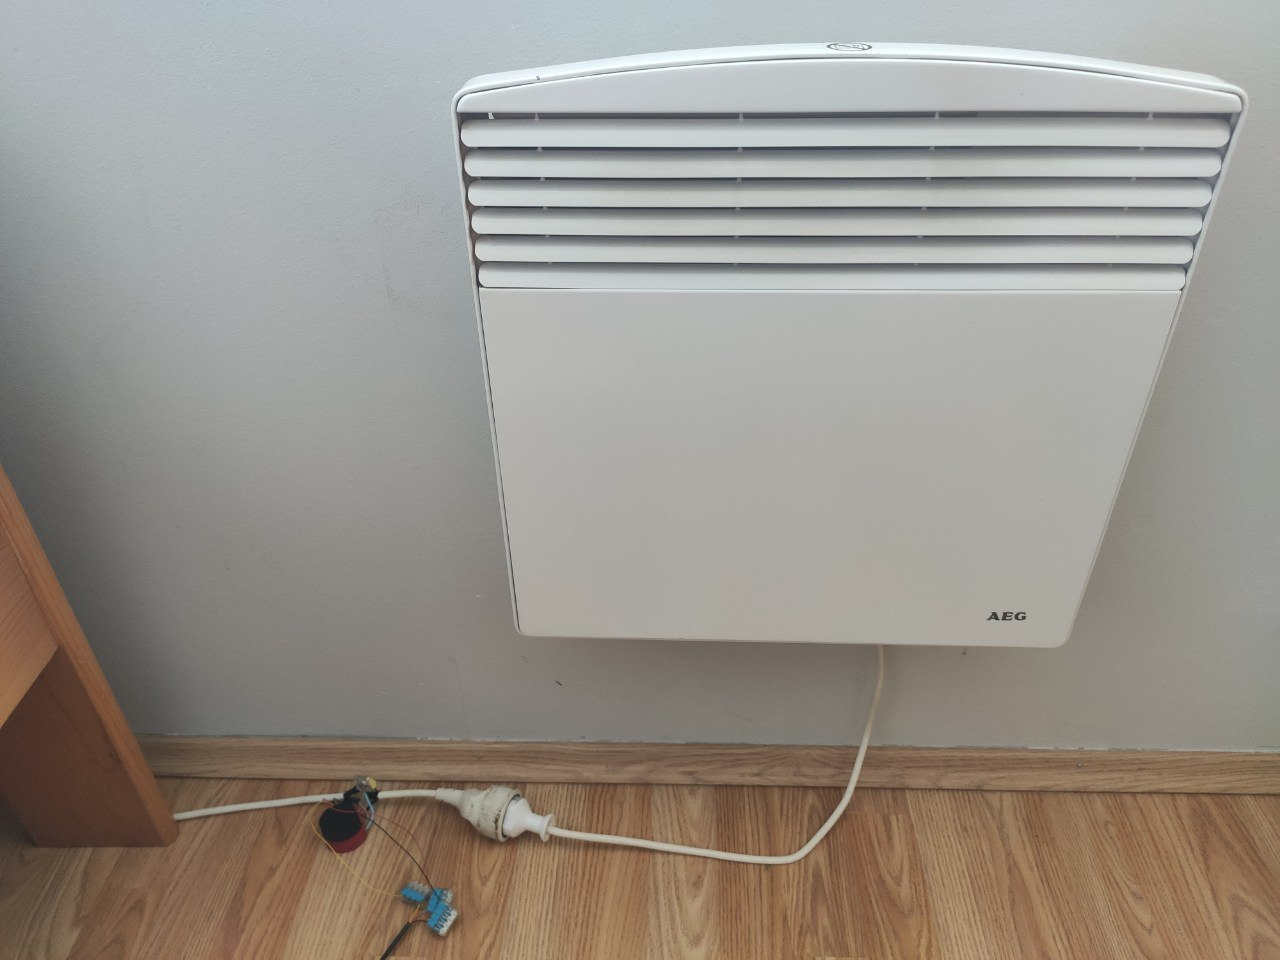
\includegraphics[width=0.37\textwidth]{obrazky-figures/aeg-wkl-1003u.png}
\caption{Fotografie instalovaného přímotopného konvektoru AEG WKL 1003 U}
\end{figure}


Konvektor AEG WKL 1003 U pracuje s pevným příkonem 1000 W, který spíná vestavěným termostatem s nastavením teploty výběrem z úrovní 1 až 7, protizámrazovou ochranu na 6 °C a volbu MAX, která by měla vytopit místnost až na 30 °C. Na pravé straně má také fyzický spínač zapnuto/vypnuto.


\section{Chytrý termostat Nest Learning}
Zajímavým zástupcem chytrých termostatů je Nest Learning Thermostat vyvíjený výrobcem Nest Labs. Dle \cite{nest} se jedná o programovatelný a samoučící se Wi-Fi termostat, který optimalizuje vytápění a chlazení domácností i podniků za účelem úspory energie. Zařízení je založeno na algoritmu strojového učení, kdy první týdny musí uživatelé regulovat termostat, aby poskytli referenční soubor dat. Termostat se pak může naučit rozvrh lidí, na jakou teplotu jsou zvyklí a kdy. Interagovat s termostatem lze klikáním a posouvání jeho ovládacího kolečka, anebo mobilní aplikací Google Home. Pomocí vestavěných senzorů a umístění telefonů se může přepnout do režimu úspory energie, když si uvědomí, že nikdo není doma.

Termostaty Nest jsou kompatibilní s většinou standardních systémů HVAC (topení, větrání a klimatizace), které využívají ústřední vytápění a chlazení. Do prostředí s přímotopnými konvektory tedy nasadit nelze.

\begin{figure}[hbt]
\centering
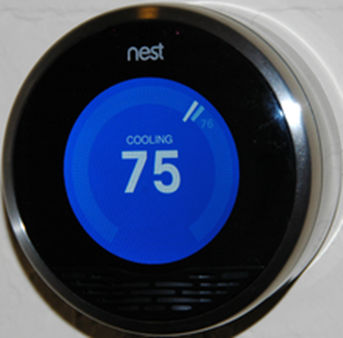
\includegraphics[width=0.4\textwidth]{obrazky-figures/nest.png}
\caption{Přední obrazovka termostatu Nest}
\end{figure}

\pagebreak

\section{Chytré elektrické přímotopy}
Na světovém trhu ovšem existují i řešení v podobě elektrických topení se zabudovanou Wi-Fi (například Nedis WIFIHTPL20FWT \cite{nedis}, který umožní vzdálené ovládání a programování pomocí aplikace Nedis SmartLife, a také podporu Amazon Alexa a Google Assistant). Toto řešení může být postačující, zásadně se však ale neodlišuje od tradičních přímotopných konvektorů a výměna jednotek v existující instalaci tedy může být zbytečně nákladná.

\begin{figure}[hbt]
\centering
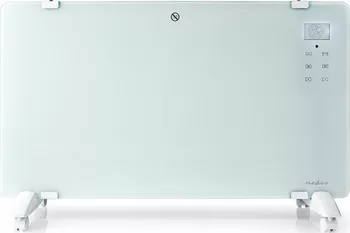
\includegraphics[width=0.6\textwidth]{obrazky-figures/nedis.png}
\caption{Wi-Fi přímotopný konvektor Nedis WIFIHTPL20FWT}
\end{figure}


\section{Tuya Wi-Fi termostat}
Posledním zajímavým produktem ve světě je Tuya Wi-Fi termostat \cite{tuyaterm}, který by svou formou byl z předchozích zmíněný nejvhodnější volbou do prostředí s existujícími přímotopnými konvektory, které bychom chtěli připojit k Wi-Fi a vzdáleně je ovládat a monitorivat. Svým hardwarovým provedením je také podobný řešení představeném v podkapitole \ref{navrh-shelly}.

\begin{figure}[hbt]
\centering
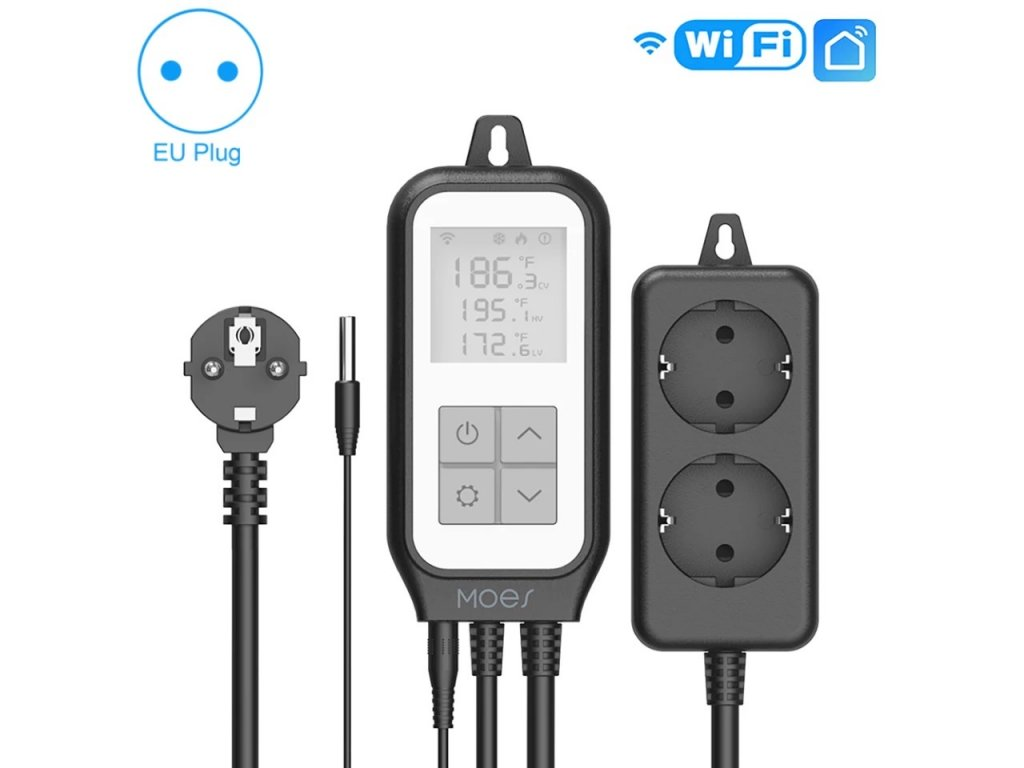
\includegraphics[width=0.56\textwidth]{obrazky-figures/tuyaterm.png}
\caption{Tuya Wi-Fi termostat}
\end{figure}


\chapter{Návrh řešení}
\label{navrh}
Tato kapitola se zabývá návrhem softwarové i hardwarové části a nastíní technologie použité pro vytvoření navrženého řešení.

\section{Shelly 1PM}
\label{navrh-shelly}
Shelly 1PM (série 1 + {\it power measurement}) je Wi-Fi relé, které bylo zvoleno pro svou nízkou cenu a širokou funkcionalitu. Umožňuje spínání zásuvky, do které je zapojen přímotop, monitorování její spotřeby ve Wattech a s pomocí přídavného modulu měřit i teplotu v místnosti. Po zapojení hardware je ve vestavěném webovém rozhraní možné toto relé připojit k domácí Wi-Fi síti a mimo jiné mu například přiřazení statické IP adresy, nastavení zdrojového napětí 110 nebo 220 V, nastavení časové zóny nebo aktualizace firmware \cite{shelly_1pm}.

Pro komunikaci se Shelly 1PM nabízí výrobce kompatibilitu s populárními platformami Android, iOS, Amazon Alexa, Google Assistant a domácí automatizační servery s použitím protokolů MQTT, CoAP a REST API \cite{shelly_1pm}. V této práci bude později využita komunikace přes rozhraní REST.

Přídavný modul teplotního senzoru \cite{shelly_tempaddon} doplňuje základní funkcionalitu relé Shelly 1 nebo 1PM o získání teploty naměřené v místnosti (dle nastavení ve °C nebo °F). K tomuto modulu je tedy ještě potřeba připojit samotný senzor DS18B20 \cite{shelly_tempsensor}, které lze připojit dokonce až 3, nebo DHT22. Pro tento projekt byl zvolen DS18B20 a bude se pracovat s teplotou ve °C.

\begin{figure}[hbt]
\centering
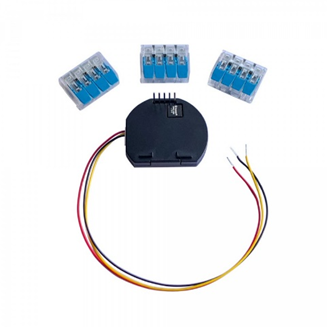
\includegraphics[width=0.33\linewidth]{obrazky-figures/shelly-tempaddon.png}
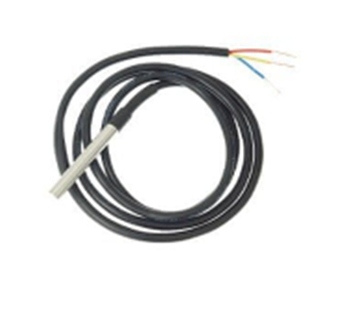
\includegraphics[width=0.33\linewidth]{obrazky-figures/shelly-tempsensor.png}
\caption{Přídavný modul pro Shelly 1/1PM a teplotní senzor DS18B20}
\end{figure}

V této práci bude použito následující zapojení, kdy relé Shelly 1PM bude vloženo do prodlužovacího kabelu, skrze který bude topení připojeno k zásuvce. Tento postup byl zvolen pro zjednodušení prvotní testovací instalace. Zařízení je jinak možné instalovat více způsoby, například přímo do zásuvky ve zdi.

\begin{figure}[hbt]
\centering
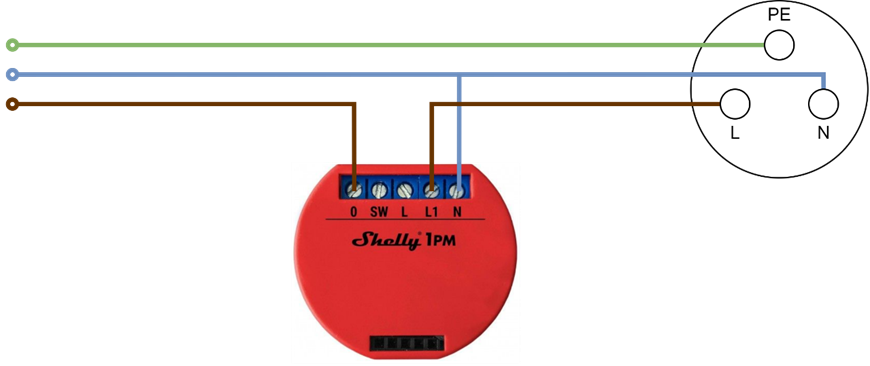
\includegraphics{obrazky-figures/shelly-diagram.png}
\caption{Diagram použitého zapojení relé Shelly 1PM}
\end{figure}

\begin{figure}[hbt]
\centering
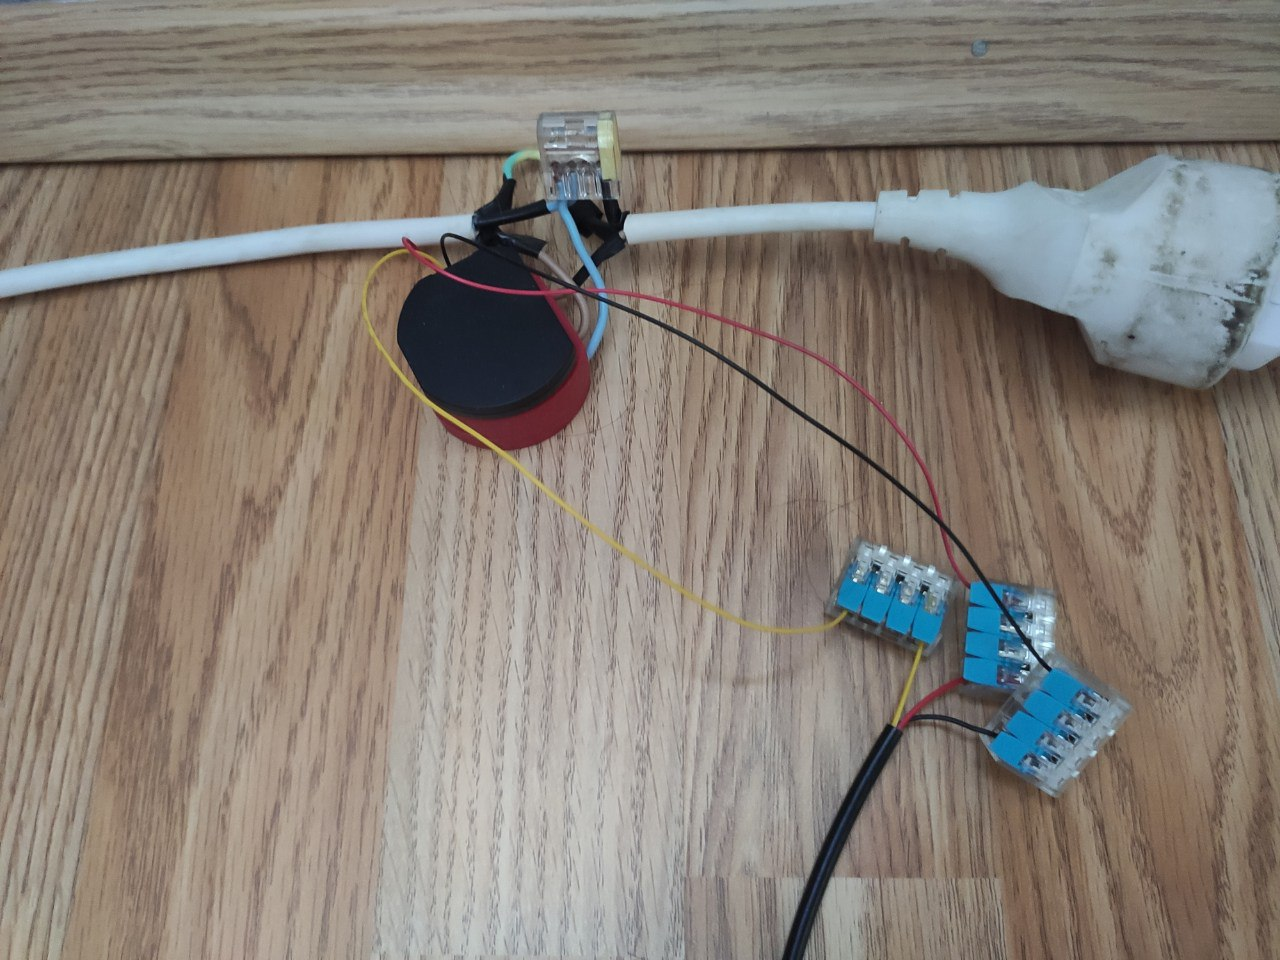
\includegraphics[width=0.44\linewidth]{obrazky-figures/shelly-photo1.png}
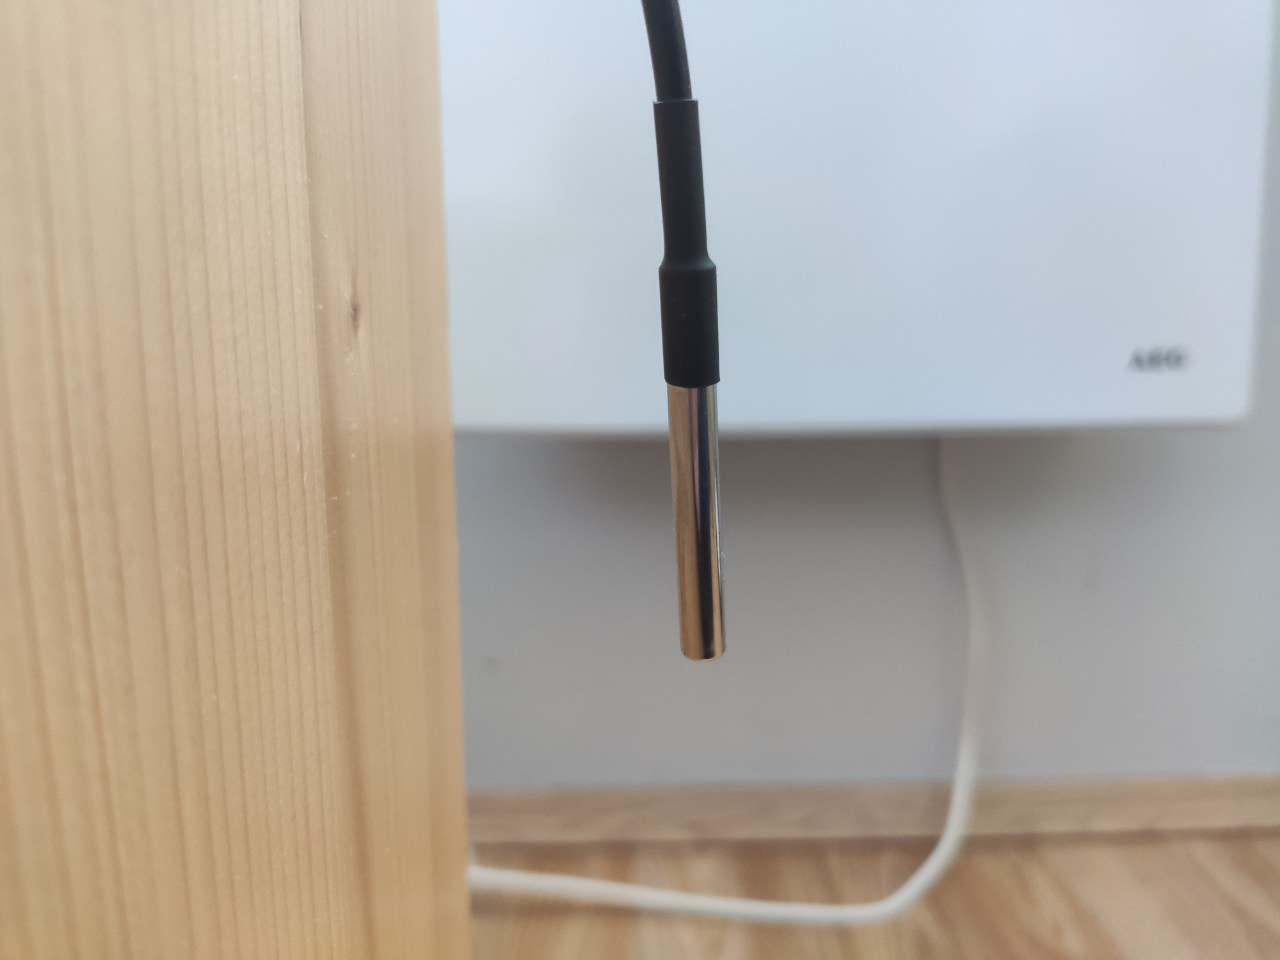
\includegraphics[width=0.44\linewidth]{obrazky-figures/shelly-photo2.png}
\caption{Fotografie instalovaného Shelly 1PM s modulem teplotního senzoru a DS18B20 umístěný v blízkosti ovládaného přímotopu}
\end{figure}

\section{Raspberry Pi 4 Model B}
Jako centrální prvek, který bude komunikovat s jednotlivými topeními připojených pomocí relé Shelly, bylo zvoleno Raspberry Pi 4 Model B ve variantě s RAM 2 GB LPDDR4 (další možné varianty jsou s 1, 4 nebo 8 GB). Dle \cite{raspberry_pi} se jedná o nejnovější a nejvýkonnější model z oblíbené řady jednodeskových počítačů Raspberry Pi. Mezi jeho klíčové vlastnosti patří výkonný 64bitový čtyřjádrový procesor, podpora dvou displejů v rozlišení až 4K prostřednictvím dvojice micro-HDMI portů, hardwarové dekódování videa až 4K 60 FPS, dvoupásmová bezdrátová LAN 2,4/5,0 GHz, Bluetooth 5.0, Gigabit Ethernet, USB 3.0 a napájení 5V DC přes USB-C, GPIO header, nebo PoE ({\it Power over Ethernet}).

Zajímavý pro použití v této práci je právě svým procesorem Broadcom BCM2711, což je 64bitové čtyřjádrové SoC ({\it System on Chip}) Cortex-A72 běžící na taktovací frekvenci 1,5 GHz \cite{raspberry_pi}. Ten by tedy pro správu připojených topení a zpracování předpovědí strojovým učením měl zajistit optimální výkon. Architektura ARM v8 je také podporována virtuálním běhovým prostědím CLR ({\it Common Language Runtime}), pod kterým bude běžet software napsaný v jazyce C\#.

\begin{figure}[hbt]
\centering
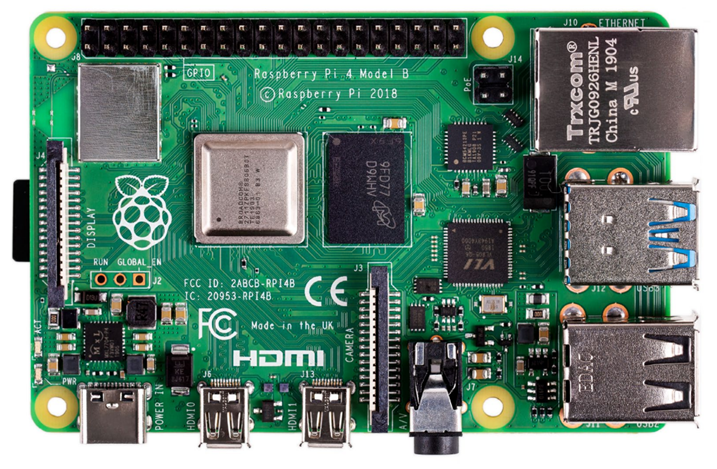
\includegraphics[width=0.66\textwidth]{obrazky-figures/raspberrypi.png}
\caption{Raspberry Pi 4 Model B}
\end{figure}

\section{C\# a platforma .NET}
Dle \cite{c_sharp} C\# je moderní objektově orientovaný a staticky typovaný programovací jazyk vytvořený společností Microsoft. Umožňuje vytvářet mnoho typů bezpečných a robustních aplikací, které běží na platformě .NET. Má své kořeny v rodině jazyků typu C a jeho syntaxe je založena na jazycích C++, Java a JavaScript. Objektový model jazyka C\# je komponentně orientovaný, což podporuje programování nezávislých a vyměnitelných modulů.

Tento jazyk také obsahuje řadu funkcí, které napomáhají vytváření robustních a odolných aplikací:

\begin{itemize}
    \item {\it Garbage Collection} automaticky uvolňuje alokovanou paměť obsazenou nedostupnými objekty
    \item {\it Nullable types} (typy s možností nabytí hodnoty null) chrání před proměnnými, které se neodkazují na alokované objekty.
    \item {\it Zpracování výjimek} poskytuje strukturovaný a rozšiřitelný přístup k detekci chyb a obnově chodu programu.
    \item {\it Lambda výrazy} podporují techniky funkcionálního programování.
    \item Syntaxe {\it LINQ (Language Integrated Query)} vytváří společný vzor pro práci s daty z jakéhokoliv zdroje.
    \item Jazyková podpora pro asynchronní operace poskytuje syntaxi pro vytváření distribuovaných systémů.
    \item Má jednotný typový systém, kde všechny typy, včetně primitivních typů jako jsou int a double, dědí z jediného kořenového typu object. Všechny typy tedy sdílí sadu běžných operací (například metoda ToString). Hodnoty jakéhokoliv typu mohou být uloženy, přemisťovány a manipulovány konzistentním způsobem. Podporuje uživatelsky definované referenční (třídy a záznamy) i hodnotové typy (struktury). Třídy kolekcí navíc obsahují iterátory, které umožňují definovat vlastní chování v klientském kódu (například v cyklech foreach).
\end{itemize}

Programy v jazyce C\# ve virtuálním systému zvaném {\it Common Language Runtime} (CLR). CLR je implementace {\it common language infrastructure} (CLI), mezinárodního standardu od společnosti Microsoft. Zdrojový kód napsaný v C\# je kompilován do {\it intermediate language} (IL), který odpovídá specifikaci CLI. Kód IL a prostředky, jako jsou řetězce a bitmapy, jsou uloženy v souborech sestavení obvykle s příponou .dll, který také obsahuje manifest s dalšími informacemi, jako jsou typy, verze programu nebo kultura (pro vícejazyčné aplikace). Když je program v C\# spuštěn, sestavení se načte do CLR, které provádí Just-In-Time kompilaci pro převod kódu z IL do nativních strojových instrukcí.

Jazyková interoperabilita je klíčovou vlastností .NET. IL kód vytvořený kompilátorem C\# odpovídá {\it Common Type Specification} (CTS). Může tedy interagovat s kódem, který byl vygenerován z .NET verzí jazyků F\#, Visual Basic, C++ a více než 20 dalších jazyků kompatibilních s CTS. Jedno sestavení může obsahovat více modulů napsaných v různých jazycích pod platformou .NET. Typy se mohou navzájem odkazovat, jako by byly napsány ve stejném jazyce.

Kromě běhových služeb zahrnuje .NET také rozsáhlé knihovny. Tyto knihovny podporují mnoho různých pracovních zátěží. Jsou uspořádány do jmenných prostorů, které poskytují širokou škálu užitečných funkcí. Knihovny zahrnují vše od vstupu a výstupu souborů přes manipulaci s řetězci až po analýzu XML, rozhraní webových aplikací až po ovládací prvky knihoven jako je Windows Forms. Typická aplikace v jazyce C\# široce využívá knihovnu tříd .NET ke zpracování běžných operací (například práce se soubory).


\section{ASP.NET Core Web API}
Serverovou částí vypracovaného řešení bude software běžící pod frameworkem {\it ASP.NET Core}. Tento framework prezentuje dle \cite{about_asp} řadu funkcí, jako je správa závislostí ({\it dependency injection}), konfigurace, {\it middleware} a další. ASP.NET Core podporuje vytváření webových aplikačních rozhraní pomocí {\it controllerů} \cite{asp_controllers} dle návrhového vzoru MVC ({\it Model-View-Controller}) nebo pomocí minimálních API. V této práci je použit přístup {\it minimálního API}, jelikož se primárně nejedná o robustní webovou aplikaci.

Aplikace vytvořené pomocí dostupných webových šablon obsahují spouštěcí kód aplikace v souboru {\it Program.cs}, kde jsou konfigurovány aplikací požadované služby a kanál ({\it pipeline}) zpracování požadavků aplikace je definován jako řada komponent middlewaru.

{\it Vkládání závislostí} (DI) zpřístupňuje nakonfigurované služby v celé aplikaci. Služby jsou přidány do kontejneru DI pomocí {\it WebApplicationBuilder.Services} jako {\it Singleton} (jediná instance dostupná v rámci celé aplikace), {\it Transient} (pro každou injekci je vytvořena nová instance třídy) a další. Služby se obvykle získávají z DI pomocí konstruktorového vkládání ({\it constuctor injection}), kde jsou služby specifikovány v parametrech konstruktoru.

Zpracování požadavků je složeno jako řada middlewarových komponent. Každá komponenta provádí operace v rámci {\it HttpContext} a buď vyvolá další middleware v kanálu, nebo ukončí požadavek. Typicky používanými middleware jsou například autorizace, vývojářská stránka s informacemi o chybách, a nebo přesměrování na HTTPS. Pomocí plánovacího middleware je v této práci také zajištěno periodické volání služeb frameworku strojového učení a databázového klienta pro ukládání záznamů o měřeních teploty.

ASP.NET Core poskytuje implementaci serveru Kestrel, který může běžet jako veřejně přístupný server vystavený přímo internetu. Kestrel je však často provozován v konfiguraci reverzní proxy se servery Nginx nebo Apache.


\section{ML.NET}
ML.NET je dle \cite{what_is_mlnet1} open-source multiplatformní framework strojového učení pro vytváření aplikací na platformě .NET v jazycích C\# nebo F\#. Obsahuje funkce jako automatizované strojové učení ({\it AutoML}) a nástroje jako {\it ML.NET CLI} a {\it ML.NET Model Builder}.

Aplikace strojového učení využívají k předpovědi vzorů v datech, místo toho aby je bylo nutné explicitně programovat. Ústředním bodem ML.NET je model strojového učení. Model specifikuje kroky potřebné k transformaci vstupních dat do predikce. ML.NET umožňuje trénovat vlastní model nebo importovat předem trénovaný model TensorFlow či ONNX.

ML.NET dle \cite{what_is_mlnet2} podporuje řadu úloh strojového učení: {\it klasifikace/kategorizace} (např. rozdělení zpětné vazby na pozitivní/negativní), {\it regrese} (předpověď spojité hodnoty, např. ceny domu na základě velikosti a lokality), {\it detekce anomálií} (např. detekce podvodných bankovních transakcí), {\it doporučení} (např. produktu na základě předchozích nákupů zákazníka), {\it časové řady} (sekvenční data, např. předpověď počasí) a {\it klasifikace obrázků} (např. kategorizace druhů rostlin).

V této práci se bude pracovat s po sobě jdoucími měřeními vývoje teploty v místnosti, které se určitým způsobem vyvíjí v čase. Jedná se tedy o časovou řadu. Analýza časových řad podporovaná frameworkem ML.NET pomáhá poskytnout odpověď na otázku budoucího vývoje teploty tím, že se podívá na historická data, identifikuje vzorce a použije tyto informace k předpovědi. Algoritmus rozhodnutí o stavu topení pracující s touto předpovědí bude popsán v kapitole \ref{implementace}.

Dle \cite{mlnet_tutorial} ML.NET pro analýzu dat používá techniku jednorozměrné analýzy časových řad. Jednorozměrná analýza časových řad se dívá na jediné numerické pozorování za určité časové období ve specifických intervalech. Framework k tomuto účelu používá algoritmus {\it analýzy singulárního spektra (SSA)}. SSA funguje tak, že rozkládá časovou řadu na sadu hlavních komponent. Tyto složky lze interpretovat jako části signálu, které odpovídají trendům, šumu, sezónnosti a mnoha dalším faktorům. Poté jsou tyto komponenty rekonstruovány a použity k předpovědi hodnot někdy v budoucnu.

\pagebreak

\section{.NET MAUI}
Pro vytvoření klientské aplikace se správou a monitorováním připojených topení bude použita knihovna .NET MAUI (Multi-platform App User Interface). Dle \cite{maui} se jedná o multiplatformní knihovnu od společnosti Microsoft, která je nástupcem aktuálního frameworku Xamarin.Forms. Umožňuje vytváření nativních mobilních a desktopových aplikací s použitím jazyků C\# a XAML podporovaný operačními systémy Android, iOS, macOS a Windows. Výhodou je tedy využití jednoho sdíleného zdrojového kódu v jednom projektu pro všechny platformy. Navíc v případě potřeby umožňuje přidání platformě specifického kódu ve specifických podadresářích, nebo pomocí direktiv překladače.

.NET 6 poskytuje řadu platformě specifických frameworků pro vytváření aplikací: .NET pro Android, .NET pro iOS, .NET pro macOS a knihovnu Windows UI 3 (WinUI 3). Všechny tyto frameworky mají přístup ke stejné knihovně základních tříd .NET 6 (BCL). Tato knihovna abstrahuje podrobnosti o základní platformě. Verze pro Android, iOS a macOS využívají implementaci .NET runtime Mono, zatímco verze pro Windows používá Win32.

Obrázek \ref{mauiArchitectureDiagra} zobrazuje architekturu aplikace používající .NET MAUI. Klientský aplikační kód typicky interaguje s .NET MAUI API (1), které poté přímo volá funkce API nativní platformy (3). Pokud je vyžadováno, funkce nativní platformy může klientský kód volat i přímo (2) \cite{maui}.

\begin{figure}[hbt]
\centering
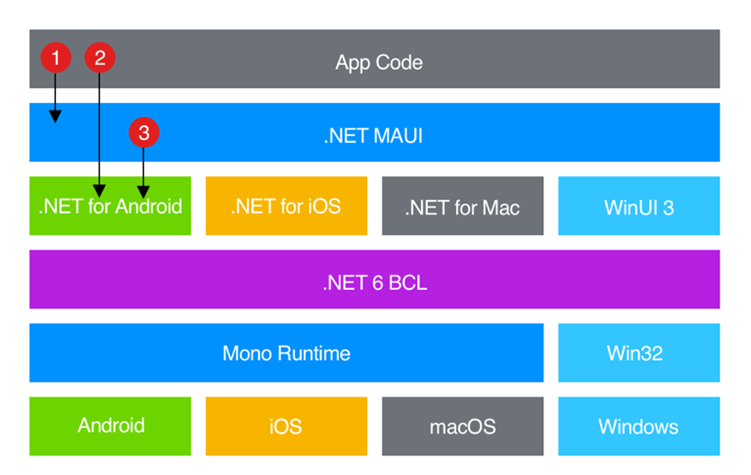
\includegraphics[width=0.7\textwidth]{obrazky-figures/maui-architecture.png}
\caption{Diagram architektury .NET MAUI}
\label{mauiArchitectureDiagra}
\end{figure}

\subsection{XAML}
Dle \cite{xaml} je XAML ({\it eXtensible Application Markup Language}) jazyk založený na XML, který je alternativou k programování kódem, kdy jsou vytvářeny instance objektů organizováné v hierarchiích. Umožňuje definovat uživatelská rozhraní aplikací pomocí značek. XAML není vyžadován v aplikaci .NET MAUI, ale je to doporučený přístup k vývoji uživatelského rozhraní, protože je často stručnější, vizuálně koherentnější a má podporu nástrojů v IDE. XAML se také dobře hodí pro použití se vzorem {\it Model-View-ViewModel (MVVM)}, kde XAML definuje pohled, který je propojen s kódem viewmodelu v C\# prostřednictvím datových vazeb.

\subsection{Model-View-ViewModel}
Návrhový vzor Model-View-ViewModel (MVVM) dle \cite{mvvm} vynucuje oddělení mezi třemi softwarovými vrstvami – uživatelským rozhraním, nazývaným pohled (view), podkladovými daty, nazývanými model, a prostředníkem mezi pohledem a modelem, nazývaným viewmodel. Pohled a viewmodel jsou často propojeny prostřednictvím datových vazeb definovaných v XAML, kde je vlastnost {\it BindingContext} obvykle instancí daného viewmodelu.

%\subsection{Uživatelské rozhraní}


\section{InfluxDB}
Pro ukládání dat o připojených topeních byla zvolen databázový software {\it InfluxDB} vytvořený společností InfluxData. Dle \cite{influx_gh} je to open-source platforma pracující s časovými řadami. To zahrnuje rozhraní API pro ukládání a dotazování nad daty, jejich zpracování pro účely monitorování a upozornění, uživatelské panely a vizualizace dat v přehledném rozgraní pod \url{http://localhost:8086/} (případně po nasazení na Raspberry Pi dostupné pod jeho IP adresou místo rozhraní localhost).

Pro zápis a dotazování nad daty nebo jakékoliv používání rozhraní API, je nejprve nutné vytvořit uživatelské přihlašovací údaje, organizaci a segment. Vše v InfluxDB je organizováno pod konceptem organizace. API je navrženo jako multi-tenant (sdílené skupinou uživatelů). Segmenty představují místo, kde jsou ukládány data časové řady.

Dotazy na tuto databázi využívají jazyka {\it Flux}. Dle \cite{flux} je to open-source funkcionální datový skriptovací jazyk určený pro dotazování, analýzu a práci s daty. Flux podporuje více typů zdrojů dat, včetně databází časových řad (jako je InfluxDB), relační SQL databáze (jako MySQL a PostgreSQL) a CSV. Flux sjednocuje kód pro dotazování, zpracování a zápis dat do jediné syntaxe.

\begin{figure}[hbt]
\centering
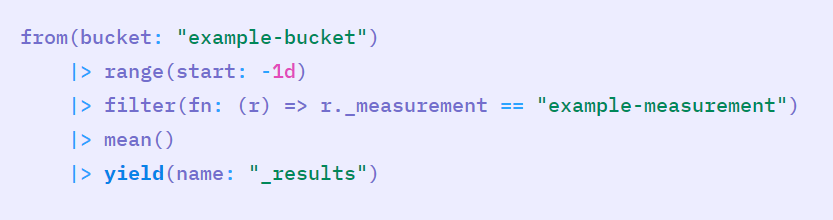
\includegraphics[width=0.75\textwidth]{obrazky-figures/flux-example.png}
\caption{Příklad dotazu pro čtení z databáze InfluxDB v jazyce Flux \cite{flux_gs}}
\end{figure}

%\noindent Více o způsobech používání funkcí API InfluxDB pro čtení a zápis v kapitole \ref{implementace}.


\section{Nginx}
Dle \cite{nginx_wiki} Nginx je softwarový webový server s managementem zátěže a reverzní proxy s otevřeným zdrojovým kódem. Pracuje s protokoly HTTP (i HTTPS), SMTP, POP3, IMAP a SSL. Zaměřuje se především na vysoký výkon a nízké nároky na paměť.

V projektu je Nginx použit dle \cite{nginx_asp} jako reverzní proxy server, který naslouchá na standardním portu 80 pro HTTP a přeposílá dotazy na ASP.NET Core server běžící na rozhraní localhost na portu 5232.

\chapter{Implementace a testování}
\label{implementace}

Tato kapitola se zabývá detaily implementace systému {\it SmartHeater} vytvořeného v rámci této práce, který je nasazen jako řídící software na dříve zmíněném minipočítači Raspberry Pi. Uživateli také umožní správu a monitorování sítě chytrých topení v jednoduché vlastní mobilní aplikaci. Závěr této kapitoly se zabývá testováním výsleků získaných během sběru dat implementovaným systémem.

\section{Architektura řešení}
Kód řešení ({\it SmartHeater}) je rozdělen na klientskou, serverovou a sdílenou část. Projekty se zdrojovým kódem řešení systému jsou rozděleny na 4 části:
\begin{itemize}
    \item \textbf{SmartHeater.Hub}: řídící hub zajišťující serverovou část pod ASP.NET Core Web API a periodické řízení a monitorování registrovaných ovladačů topení.
    \item \textbf{SmartHeater.ML}: knihovna tříd nad frameworkem ML.NET pro strojové učení.
    \item \textbf{SmartHeater.Maui}: klientská multiplatformní aplikace nad .NET MAUI.
    \item \textbf{SmartHeater.Shared}: knihovna tříd obsahující sdílené prostředky používané řídícím hubem i mobilní aplikací (například výčtové typy a třídy použité v HTTP komunikaci pro serializaci a deserializaci ve formátu JSON).
\end{itemize}

\begin{figure}[hbt]
\centering
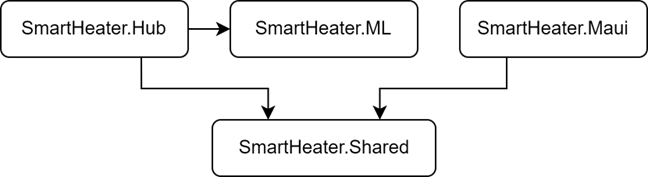
\includegraphics[width=0.75\textwidth]{obrazky-figures/smartheater-architecture.png}
\caption{Graf závislostí mezi projekty řešení}
\end{figure}

\pagebreak

\section{Řídící hub}
Centrálním bodem této práce je software běžící na Raspberry Pi, které zde má roli hlavního řídícího hubu. Cílem této části je správa, ovládání a monitorování připojených topení a poskytnutí rozhraní webového API pro komunikaci s klientskou aplikací. Jádrem je projekt {\it SmartHeater.Hub}. V souboru {\it Program.cs} má nakonfigurováno zajištění vytrénování modelu ML, registraci služeb dále poskytnuté DI kontejnerem, plánovač poskytnutý knihovnou {\it Coravel} \cite{coravel}, který periodicky spuští kód tříd ze složky {\it Invocables}, ladící prostředí {\it Swagger} a HTTP koncové body poskytovaného webového API.

\begin{figure}[hbt]
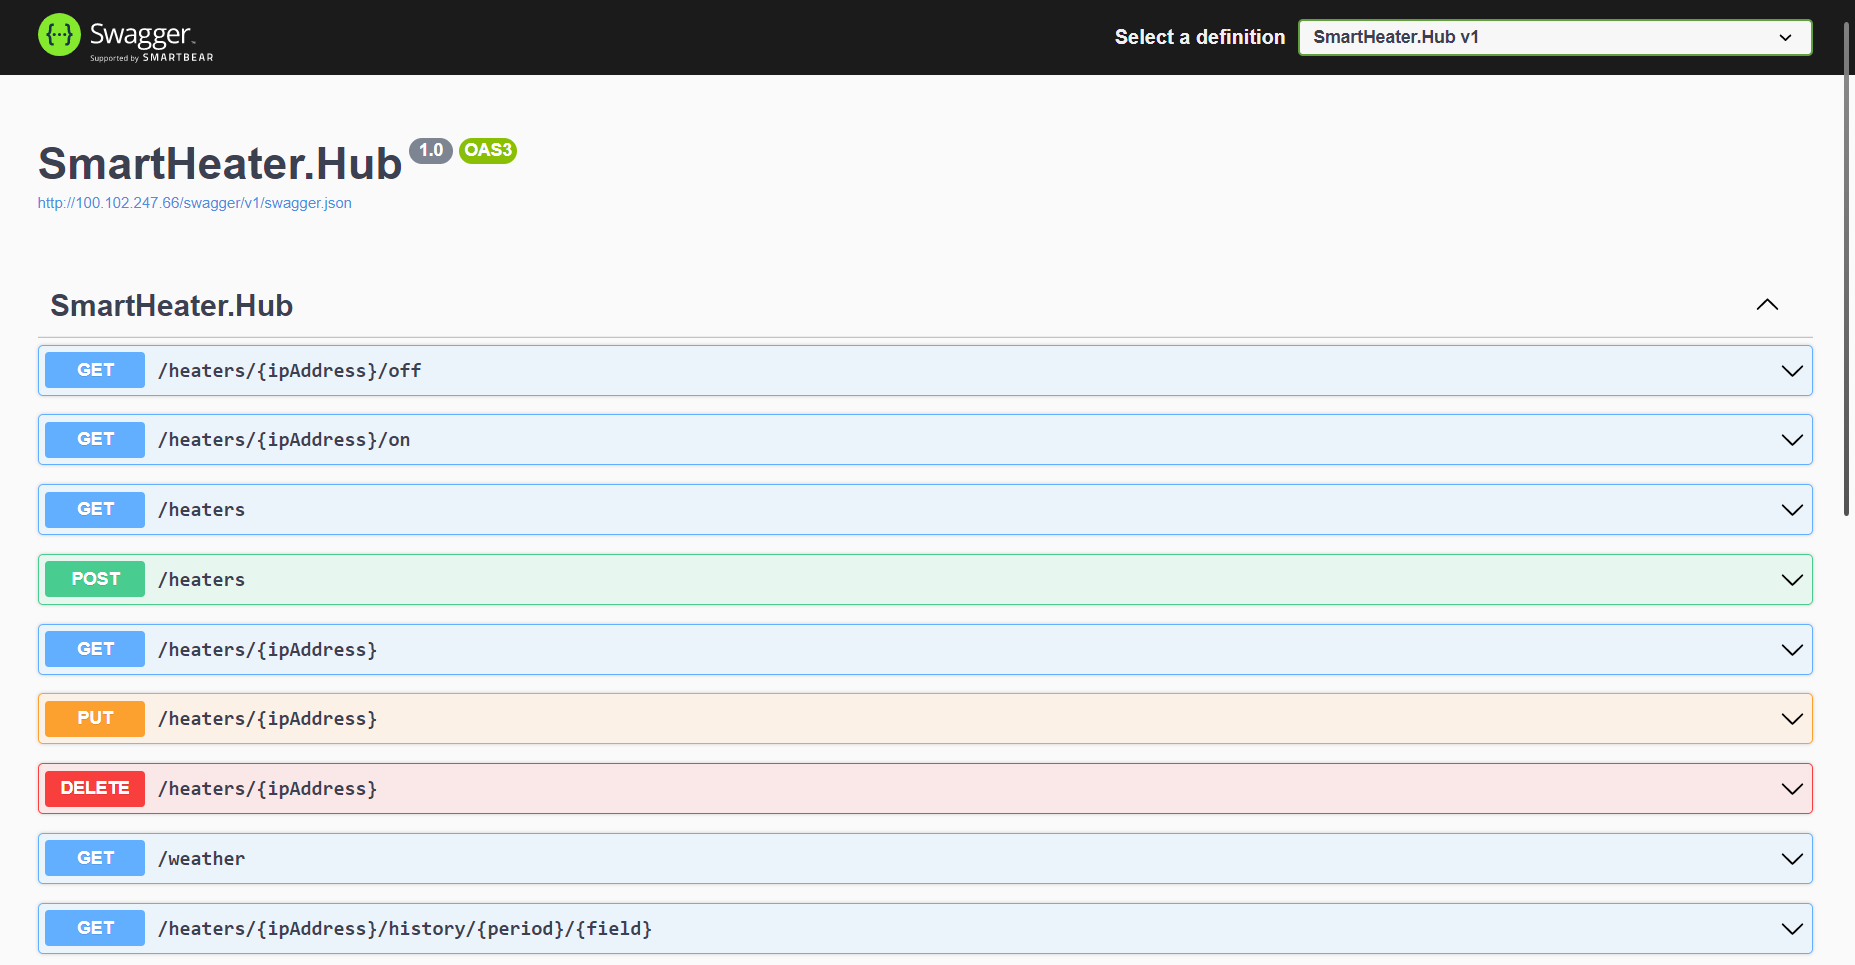
\includegraphics[width=\textwidth]{obrazky-figures/swagger.png}
\caption{Prostředí Swagger pro ladění koncových bodů webového API}
\end{figure}

Rozhraní pro registrované služby a pro každé z nich jedna z možných implementací se v projektu nacházejí ve jmenném prostoru {\it SmartHeater.Hub.Services}. Způsob práce s využitím rozhraní byl zvolen z důvodu možnosti budoucí rozšiřitelnosti a nahrazení aktuální implementace bez nutnosti přepisování kódu, který rozhraní využívá.

\begin{figure}[hbt]
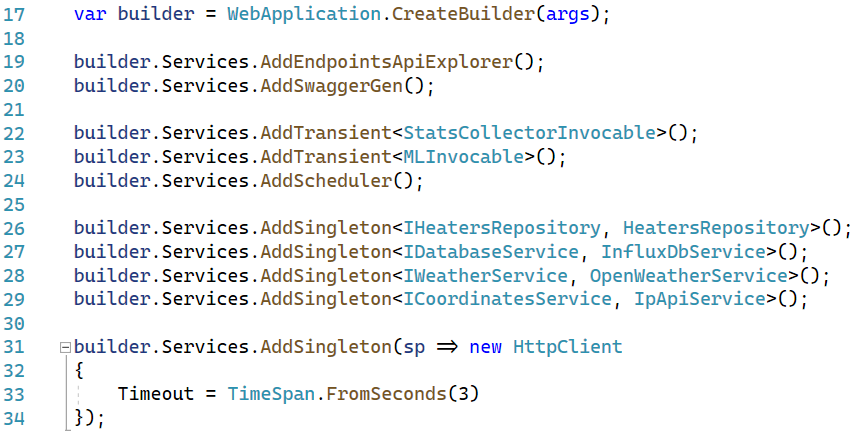
\includegraphics[width=0.69\textwidth]{obrazky-figures/code-hubservices.png}
\caption{Registrace implementací rozhraní služeb v souboru {\it Program.cs}, které bude DI kontejner poskytovat v rámci aplikace}
\end{figure}

\subsection{Data o počasí}
Pro sledování vlivu počasí na teplotu uvnitř v místnosti bylo do projektu přidáno rozhraní {\it IWeatherService}, které zprostředkovává metody pro čtení teploty ve °C i °F (v této práci se primárně pracuje se °C). Pro pohodlí uživatele bylo také přidáno rozhraní {\it ICoordinatesService}, které umožňuje automatické zjištění polohu zařízení, která bude použita k získání dat o počasí z daného místa.

Implementace ve třídě {\it IpApiService} k tomuto využívá webovou službu \url{https://ipapi.co/}, která vrací souřadnice dle veřejné IP adresy zařízení. Tyto souřadnice jsou uloženy v poli, aby se zamezilo zbytečnému síťovému provozu. Pracuje se zde tedy s předpokladem, že zařízení, na kterém software poběží, typu Raspberry Pi bude instalováno na jednom místě a nebude měnit svou polohu.

Samotné rozhraní pro získávání dat o počasí implementuje třída {\it OpenWeatherService}. Jako zdroj používá volně dostupné webové API \textbf{OpenWeather}, které pro svůj provoz vyžaduje pouze registraci a vytvoření API klíče. Získaný klíč je následně uložen do souboru {\it appsettings.json}. Tento soubor obsahuje konfiguraci pro ASP.NET projekt, ze které lze snadno číst pomocí vestavěného rozhraní {\it IConfiguration}.

\begin{figure}[hbt]
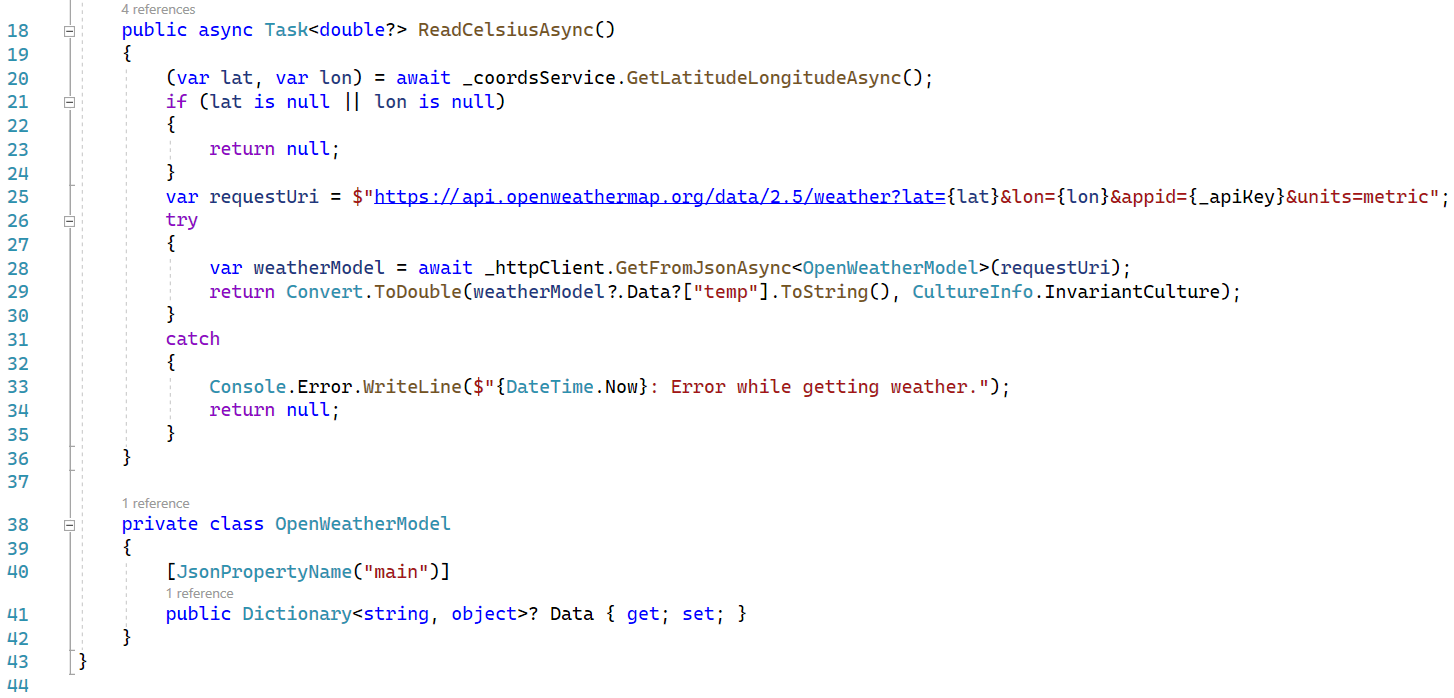
\includegraphics[width=1.05\textwidth]{obrazky-figures/code-openweather-read.png}
\caption{Metoda {\it ReadCelsiusAsync} pro získání souřadnic aktuální polohy zařízení volá službu {\it ICoordinatesService}, které použije v HTTP požadavku na službu {\it OpenWeather}. Získaná data ve formátu JSON jsou deserializována do privátní třídy (zde je důležitá položka {\it ''main''}, jejíž položky jsou mapovány na slovník). Ze slovníku {\it Data} je z položky {\it ''temp''} vyčtena teplota ve °C a vrací se jako hodnota typu double. V případě chyby je vrácena hodnota null.}
\end{figure}

\pagebreak

\subsection{Databázové rozhraní}
Rozhraní {\it IDatabaseService} zprostředkovává připojení k databázi. Obsahuje metody pro zápis měření (jako parametry vyžaduje záznam stavu topení a počasí) a čtení historie (vrací kolekci databázových záznamů pro konkrétní model topení ve vybraném období a z vybraného sloupce tabulky v databázi).

Implementace ve třídě {\it InfluxDbService} využívá knihovnu {\it InfluxDB.Client} poskytující třídy pro práci s databázovým systémem InfluxDB. Podobně jako v předchozí podkapitole používá {\it InfluxDbService} konfiguraci uloženou v souboru {\it appsettings.json}, kde má uložený název organizace a segmentu, které je třeba nastavit v databázi InfluxDB po její instalaci, a databázovým systémem vygenerovaný přístupový token.

\begin{figure}[hbt]
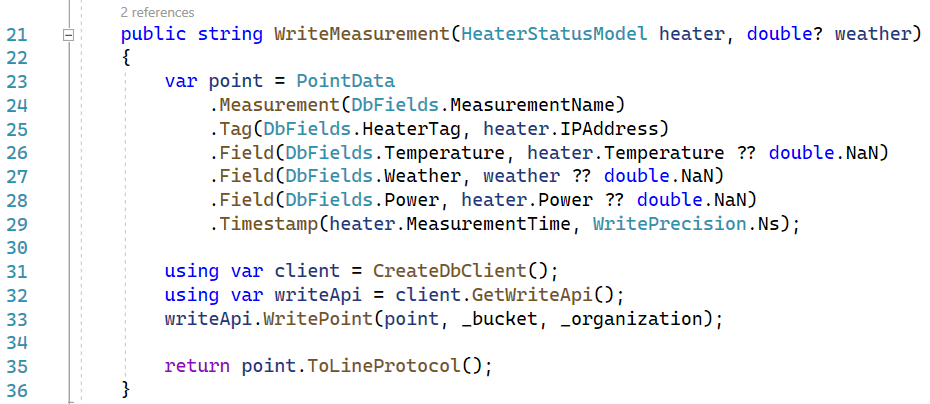
\includegraphics[width=0.68\textwidth]{obrazky-figures/code-influx-write.png}
\caption{Metoda {\it WriteMeasurement} zapisuje záznam o měření stavu topení a počasí vytvořením objektu s daty s položkami daného měření a časovou značkou. Klient InfluxDB obsahuje zapisovací API, které daný bod zapíše do databáze dle nakonfigurované organizace a segmentu.}
\end{figure}

\begin{figure}[hbt]
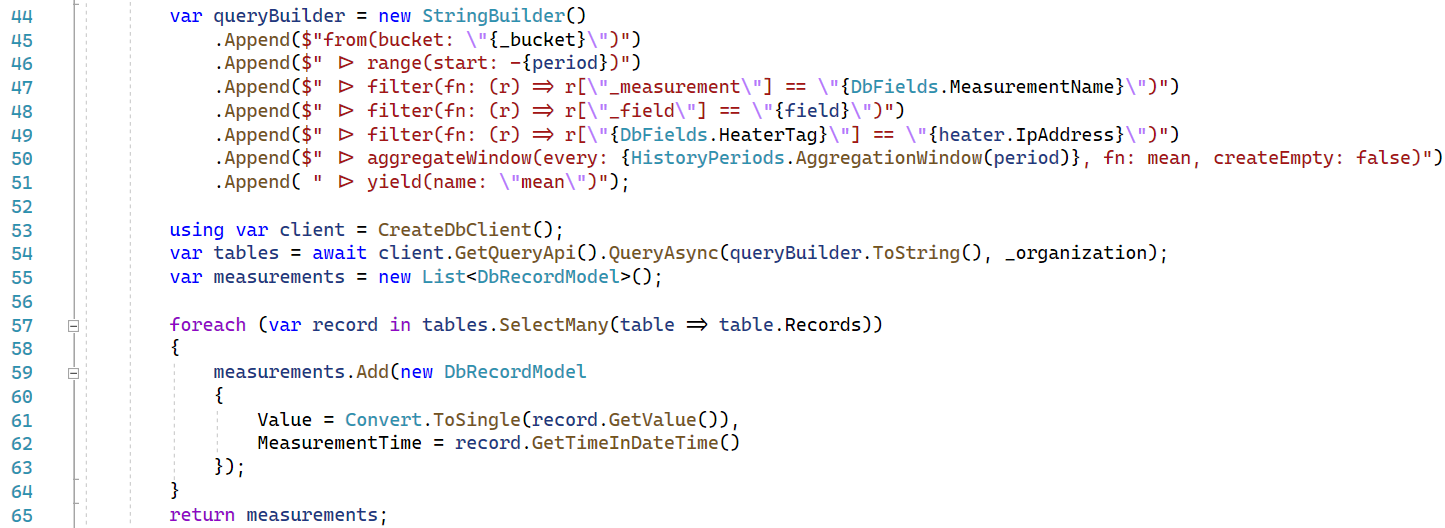
\includegraphics[width=1.05\textwidth]{obrazky-figures/code-influx-read.png}
\caption{Část metody {\it ReadHistoryAsync}, kde je vytvořen dotaz v jazyce Flux, kterým získá data ze zadaného časového období a vybraného sloupce databázové tabulky pro zvolené topení, které je filtrované dle své IP adresy. Získané záznamy jsou navráceny v kolekci s objekty typu {\it DbRecordModel}. Jedná se o vlastní model, který je dále využíván v rámci implementace mobilní aplikace. Obsahuje hodnotu měření typu float a časové razítko.}
\end{figure}

\pagebreak
Jmenný prostor {\it SmartHeater.Shared.Static} obsahuje pomocné statické třídy {\it DbFields} a {\it HistoryPeriods} zajišťují kontrolu validity vyžádané položky databáze a časového úseku. K tomuto používají předdefinované konstanty typu string. Obsahují metodu {\it GetAll} sloužící jako iterátor přes všechny definované konstanty a metodu {\it IsValid}, která zjistí validitu zadaného parametru porovnáním jeho existence s položkami iterátoru {\it GetAll}.

\begin{figure}[hbt]
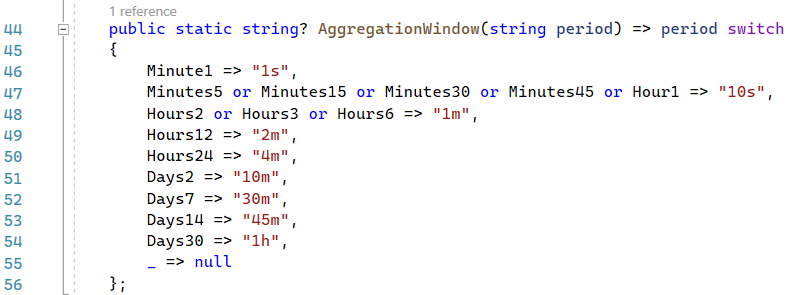
\includegraphics[width=0.75\textwidth]{obrazky-figures/code-aggregationwindow.png}
\caption{Třída {\it HistoryPeriods} navíc pro část Flux dotazu obsahuje metodu {\it AggregationWindow}, která pro dané časové období (dle odpovídající definované konstanty) vrací příslušnou velikost agregačního okna. Tyto velikosti byly odvozeny od velikostí okna, které používá webové rozhraní InfluxDB pro dané časové úseky. Delší vyžádané časové období představuje více naměřených hodnot a s tím spojené vyšší nároky na paměť a síťový provoz.}
\end{figure}


\subsection{Správa a ovládání topení}
Rozhraní {\it IHeatersRepository} poskytuje metody pro správu sítě topení. Umožňuje získání informací o registrované jednotce ({\it GetHeaterAsync}) i možnost získání detailu s měřením teploty v místnosti a spotřeby energie ({\it GetHeaterDetailAsync}), čtení i zápis kolekce registrovaných jednotek ({\it ReadHeatersAsync} a {\it WriteHeatersAsync}), vkládání ({\it InsertAsync}), aktualizace ({\it UpdateAsync}) a mazání jednotlivých topení ({\it DeleteAsync}), a získání služby implementující rozhraní {\it IHeaterControlService} pro ovládání daného topení (pro všechny registrované jednotky {\it GetHeaterServicesAsync}, nebo pro jedno konktrétní registrované topení {\it GetHeaterService} a {\it GetHeaterServiceAsync}).
 
Implementace ve třídě {\it HeatersRepository} pracuje s kolekcí topení uloženou v souboru {\it heaters.json} (a pokud neexistuje, vytvoří si jej). Běžně by bylo vhodné je ukládat jako databázové entity, ale použitá databáze InfluxDB pracuje pouze s časovými řadami, pro které je optimalizovaná, a instalovat vedle ní navíc relační databázový server by bylo v případě tohoto projektu zbytečné.

Jmenný prostor {\it SmartHeater.Shared.Models} obsahuje třídy použitých datových modelů. Jedním z nich je {\it HeaterListModel} představující model registrovaného topení. Topení jsou rozlišována dle \textbf{IP adresy}. Dále model obsahuje informace o názvu topení, typu topné jednotky (výčtový typ {\it HeaterTypes} aktuálně obsahuje pouze {\it Shelly1PM}, ale do budoucna je možné řešení rozšířit i o další typy), a nastavené referenční teplotě, kterou se bude ovládající část snažit v místnosti udržet.

\pagebreak

\begin{figure}[hbt]
\centering
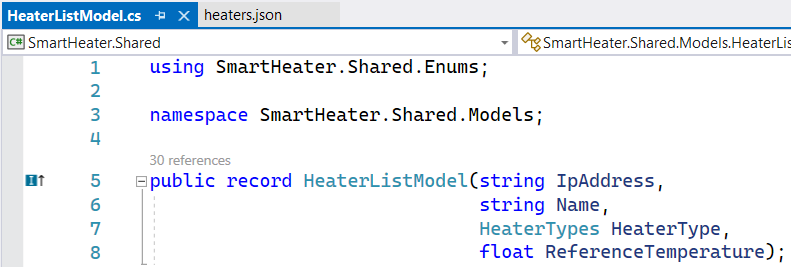
\includegraphics[height=2.94cm]{obrazky-figures/code-heaterslistmodel.png}
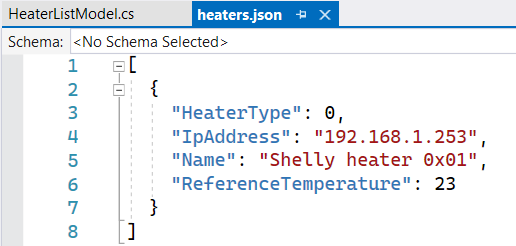
\includegraphics[height=2.94cm]{obrazky-figures/code-heatersjson.png}
\caption{{\it HeaterListModel} a reprezentace jejich kolekce ve formátu JSON uložené v souboru {\it heaters.json}}
\end{figure}

Dalším datovým modelem je {\it HeaterStatusModel}, který představuje záznam o stavu topení. Obsahuje informace, zda je topení ve stavu zapnuto nebo vypnuto, naměřenou teplotu v místnosti, záznam o okamžité spotřebě elektrické energie ve Wattech a časové razítko měření. Model použitý pro získání detailu o topení {\it HeaterDetailModel} obsahuje informace uložené v rámci {\it HeaterListModel} i záznam o měření v položce typu {\it HeaterStatusModel}.

Oddělené rozhraní ovladače topení {\it IHeaterControlService} obsahuje metody pro zapnutí ({\it TurnOnAsync}) i vypnutí ({\it TurnOffAsync}) topné jednotky a získání jejího stavu ({\it GetStatusAsync}) v modelu {\it HeaterStatusModel}.

\begin{figure}[hbt]
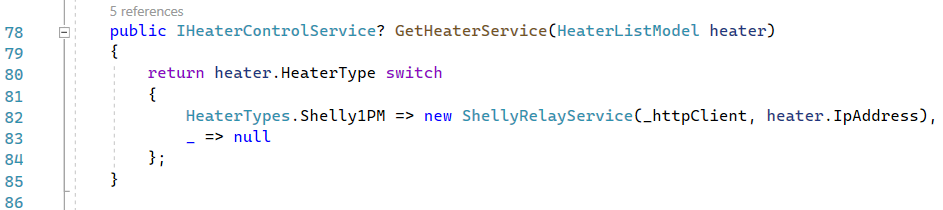
\includegraphics[width=0.9\textwidth]{obrazky-figures/code-heaterservice-decode.png}
\caption{Metoda třídy {\it HeatersRepository} vracející příslušnou implementaci rozhraní {\it IHeaterControlService} dle konkrétního typu topení. Pro neznámý neimplementovaný typ vrací hodnotu null. V této práci je však použito výhradně zařízení Shelly 1PM, pro které je implementace rozhraní {\it IHeaterControlService} vytvořena ve třídě {\it ShellyRelayService}. Ta stojí na komunikaci s vestavěným lokálním REST API \cite{shelly_api}, a proto je vyžadována konfigurace IP adresy zařízení.}
\end{figure}

\pagebreak

\begin{figure}[hbt]
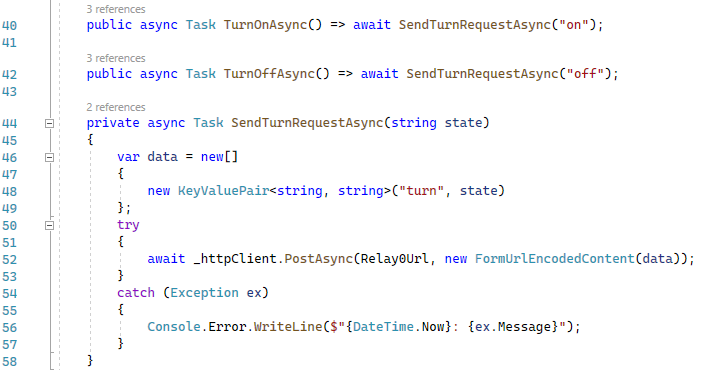
\includegraphics[width=0.8\textwidth]{obrazky-figures/code-shellyturns.png}
\caption{Třída {\it ShellyRelayService} obsahuje metody {\it TurnOnAsync} a {\it TurnOffAsync} využívají k zasílání příslušného příkazu zapnout/vypnout HTTP metodu {\it POST} na koncový bod \textbf{/relay/0}, jíž je v těle zprávy předán příkaz {\it ''turn'' ''on''} nebo {\it ''off''} ve formátu {\it application/x-www-form-urlencoded} dle \cite{shelly_http}.}
\end{figure}

\begin{figure}[hbt]
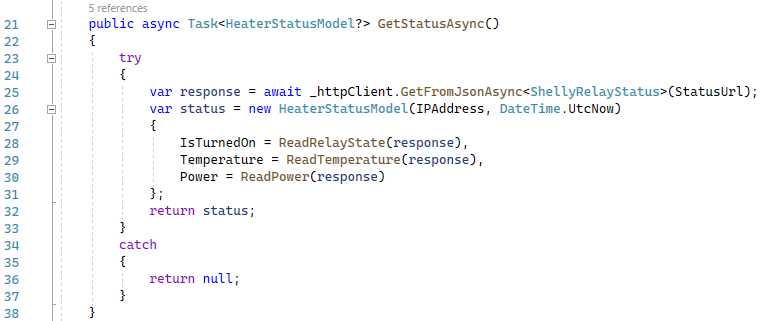
\includegraphics[width=0.88\textwidth]{obrazky-figures/code-shelly-status.png}
\caption{Metoda {\it GetStatusAsync} získá data o stavu zařízení Shelly použitím HTTP metody {\it GET} na koncový bod \textbf{/status}. Obsah odpovědi ve formátu JSON je deserializován do privátní třídy {\it ShellyRelayStatus}, jejíž položky následně dekóduje do objektu typu {\it HeaterStatusModel} voláním pomocných metod.}
\end{figure}

\noindent Třída {\it ShellyRelayStatus} mapuje dle \cite{shelly-api-status} následující položky JSON odpovědi:
\begin{itemize}
    \item {\it ''relays''}: Jedná se o seznam relé a obsahuje položky s jejich stavem (Shelly 1PM obsahuje pouze jedno relé, takže čteme z první položky). Položkou je zde slovník, ze kterého lze z položky {\it ''ison''} vyčíst, zda je relé ve stavu zapnuto nebo vypnuto.
    \item {\it ''ext\_temperature''}: Jedná se o seznam přípojených externích teplotních senzorů (v této práci je pro každé topení brán v potaz pouze jeden senzor, takže opět čteme z první položky). Položkou je zde slovník z jehož položky {\it ''tC''} vyčteme teplotu ve °C.
    \item {\it ''meters''}: Obsahuje informace o naměřené okamžité spotřebě elektrické energie ve Wattech, jejíž hodnota je vyčtena z položky {\it ''power''}.
\end{itemize}

\pagebreak

\subsection{Komunikace klient-server}
Klientská aplikace může komunikovat s řídícím hubem pomocí HTTP metod dle registrovaných koncových bodů na dostupném webovém API ASP.NET Core.

\begin{figure}[hbt]
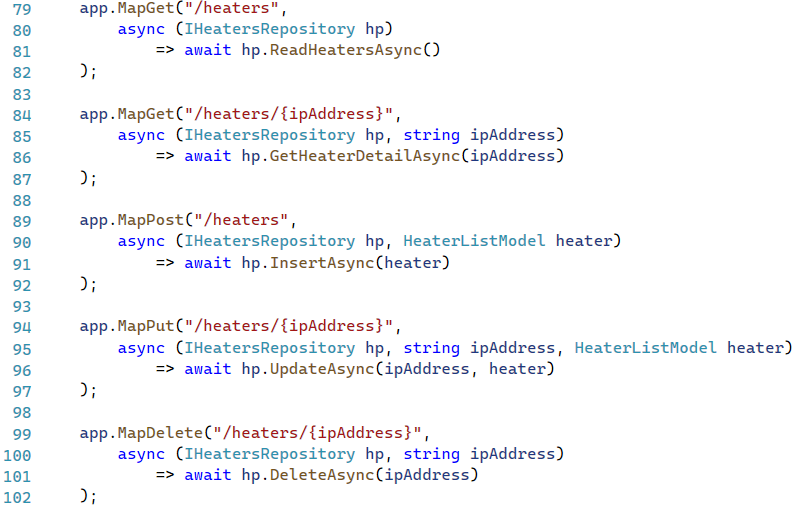
\includegraphics[width=0.75\textwidth]{obrazky-figures/code-endpoints.png}
\caption{Příklad způsobu registrace HTTP metod pomocí minimálního webového API v souboru {\it SmartHeater.Hub/Program.cs}. V implementaci jsou použity HTTP metody {\it GET}, {\it POST}, {\it PUT} a {\it DELETE}. Tyto koncové body využívají služby poskytované DI kontejnerem. Na poskytnuté instanci služby jsou volány její asynchronní metody.}
\end{figure}

\noindent Dle zvolené HTTP metody koncové body poskytují následující činnosti:
\begin{itemize}
    \item {\it ''/heaters''}: Požadavkem metodou {\it GET} vrací kolekci registrovaných topení typu {\it HeaterListModel}. Metoda {\it POST} naopak {\it HeaterListModel} očekává v těle zprávy s vyplněnými informacemi o novém topení, které přidá do kolekce a uloží do souboru {\it heaters.json}.
    \item {\it ''/heaters/\{ipAddress\}''}: Metoda {\it GET} pro tento koncový bod vrací detailní informace o topení v modelu {\it HeaterDetailModel}. Požadavek metodou {\it PUT} upraví specifikovaný záznam o topení přijatým {\it HeaterListModel} v těle zprávy. Dále metodou {\it DELETE} smaže specifikované topení z kolekce uložené v souboru {\it heaters.json}.
    \item {\it ''/weather''}: Požadavkem metodou {\it GET} vrací záznam o aktuální venkovní teplotě ve °C získaném ze služby {\it OpenWeather}.
    \item {\it ''/heaters/\{ipAddress\}/history/\{period\}/\{field\}''}: Metoda {\it GET}, která vrací historii uloženou v databázi InfluxDB, která je filtrována v dotaze v jazyce Flux dle topení specifikovaného IP adresou, požadovaným časovým úsekem a typem položky databáze.
    \item {\it ''/periods''}: Vrací kolekci podporovaných časových úseků pro filtrování Flux dotazem specifikované ve statické třídě {\it HistoryPeriods}.
    \item {\it ''/fields''}: Vrací kolekci v implementaci použitých položek uložených v databázi InfluxDB (sloupce tabulky). 
    \item {\it ''/smartheater-availability-test''}: Používaný mobilní aplikací pro snadné zjištění dostupnosti serveru.
\end{itemize}


\section{Mobilní aplikace}
Multiplatformní aplikace implementovaná nad frameworkem .NET MAUI byla vytvořena jako klient pro komunikaci se serverem běžícím pod frameworkem ASP.NET a umožní uživateli snadnou správu a monitorování sítě topení instalovaných v domácnosti.

Ústředním bodem zdrojového kódu aplikace je její konfigurace v souboru {\it MauiProgram.cs}. Zde je podobně jako v konfiguraci řídícího hubu poskytován kontejner DI, který poskytuje stránky, viewmodely a další služby (například {\it HttpClient} pro komunikaci s webovým API). Další konfigurace zdrojů pro XAML se nacházi v souborech {\it App.xaml} a {\it App.xaml.cs}.

Jako základní prvek propojující uživatelské rozhraní této aplikace je použit {\it Shell}, který dle \cite{maui-shell} snižuje složitost vývoje aplikací tím, že poskytuje základní funkce vyžadované většinou aplikací, včetně jediného místa pro popis vizuální hierarchie aplikace, navigační schéma založené na URI, které umožňuje navigaci na jakoukoli stránku v aplikaci a integrovaný obslužný program vyhledávání.

\begin{figure}[hbt]
\label{appshellprovider}
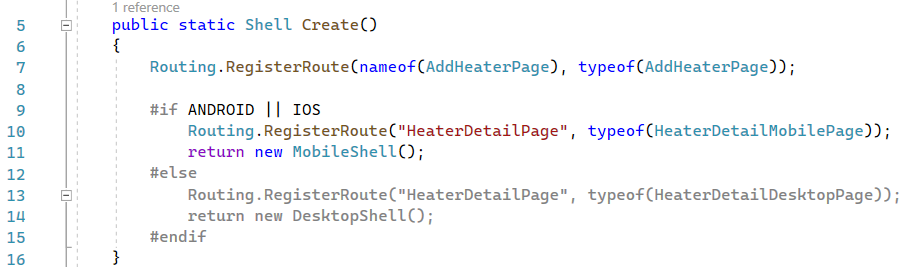
\includegraphics[width=0.87\textwidth]{obrazky-figures/code-maui-appshellprovider.png}
\caption{Statická třída {\it AppShellProvider} ze jmenného prostoru {\it SmartHeater.Maui.Providers} zprostředkovává hlavní rozhraní aplikace vestavěného typu {\it Shell}. Využívá možností direktiv pro překladač, kdy pomocí definovaných proměnných běhového prostředí lze zjistit, zda je překládáno pro mobilní či desktopovou platformu. Dle toho vrací {\it MobileShell} nebo {\it DesktopShell}, které jsou definovány ve složce {\it Pages}, a také upravuje směrování na příslušnou stránku detailu topení, jejíž rozhraní je také upraveno dle platformy.}
\end{figure}

Zdrojový kód aplikace obsahuje také platformě specifický kód ve složce {\it Platforms}. V rámci této práce byla testována pouze verze pro Windows, kde nebylo oproti vytvořené šabloně potřeba nic měnit, a platformu Android, pro kterou byl upraven pouze soubor {\it AndroidManifest.xml} přidáním vyžadovaných systémových oprávnění pro přístup k síťovému rozhraní zařízení.

Verze pro platformy {\it iOS}, {\it Mac Catalyst} a {\it Tizen} nebyly v rámci této práce otestovány, kvůli nemožnosti přístupu k potřebnému hardware (smartphony {\it Apple iPhone} a počítače {\it Mac}). Díky vlastnostem použitého frameworku .NET MAUI a sdíleného zdrojového kódu lze ale předpokládat jejich plnou funkčnost.

Samotný sdílený kód stránek aplikace v jazyce XAML se nachází ve složce {\it Pages}. Všechny dodržují návrhový vzor MVVM, kdy hlavní značka stránky {\it ContentPage} má specifikovaný svůj datový typ viewmodelu specifikovaný v parametru {\it x:DataType}. Toto umožňuje použití prvků viewmodelu pro datové vazby v XAML značkách nižší úrovně. V příslušném xaml.cs souboru je v parametru konstruktoru třídy stránky specifikován vyžadovaný viewmodel a přiřazen vlastnosti {\it BindingContext}. Po spuštění je instance objektu viewmodelu poskytnuta DI kontejnerem.

\begin{figure}[hbt]
\centering
\frame{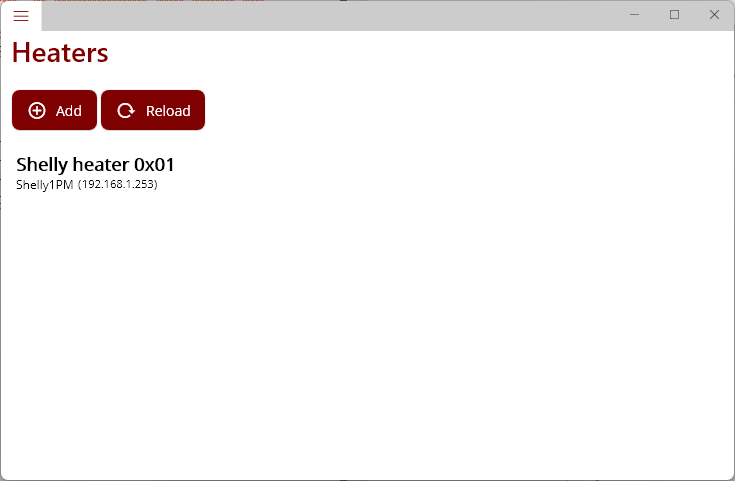
\includegraphics[height=7.1cm]{obrazky-figures/screenshots/1-windows.png}}
\frame{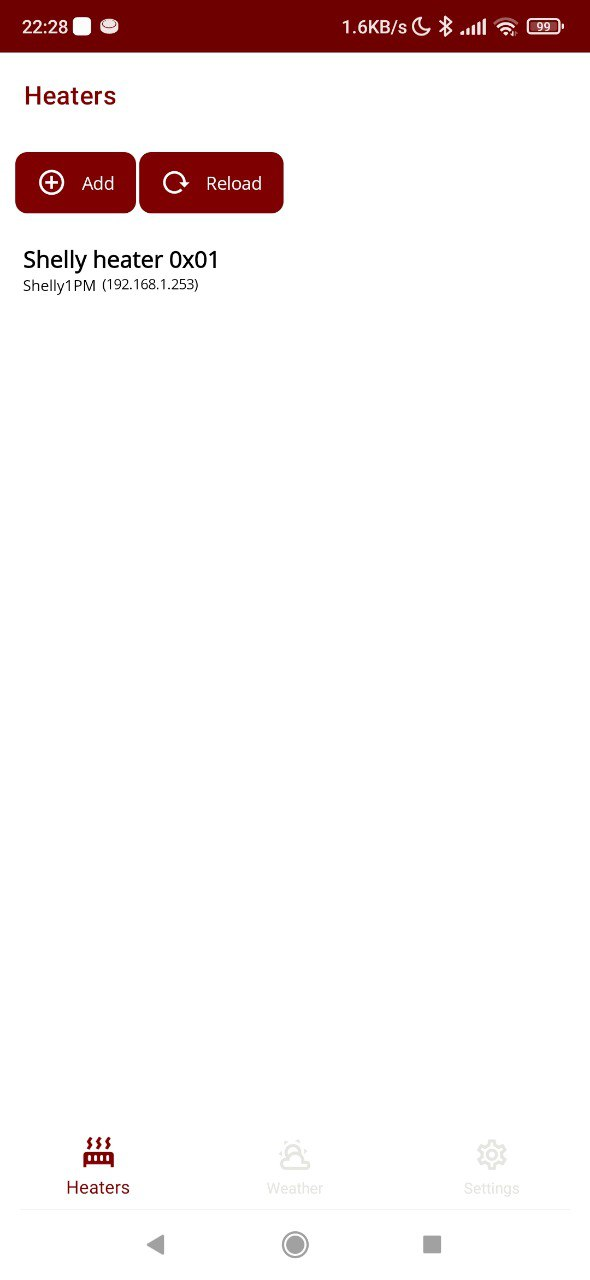
\includegraphics[height=7.1cm]{obrazky-figures/screenshots/1-android-tabbar.png}}
\caption{Ukázka použití {\it DesktopShell} pro Windows, který pro navigaci aplikace používá {\it Flyout} hamburger menu, a {\it MobileShell} pro Android, který používá navigaci pomocí záložek {\it TabBar}. Úvodní stránka aplikace zobrazuje seznam registrovaných topných jednotek (v případě testovací instalace je zobrazeno jedno zařízení Shelly 1PM).}
\end{figure}

\subsection{Stránky pro správu topení}
Zobrazení seznamu registrovaných topení se nachází v souboru {\it HeatersPage.xaml}. Krom kolekce zobrazeném v XAML značce {\it CollectionView} obsahuje také tlačítka pro přidání topení a znovunačtení seznamu (využívá se například po prvotním spuštění, kdy ještě nebyla nakonfigurována IP adresa řídícího hubu na stránce nastavení).

Stránka pro přidání topení {\it AddHeaterPage} obsahuje textová pole pro prvky třídy {\it HeaterListModel}, která je součástí kódu sdíleného mezi mobilní aplikací a řídícím hubem. Vyplněná instance {\it HeaterListModel} je v metodě viewmodelu {\it AddHeaterViewModel} serializována do formátu JSON a odeslána na webové API řídícího hubu pomocí HTTP metody {\it POST}. Toto jedno uživatelské rozhraní lze znovupoužít i pro editaci jednotky pomocí {\it Shell} podporované URI navigace. V případě editace je pro uložení použita metoda {\it PUT}.

\begin{figure}[hbt]
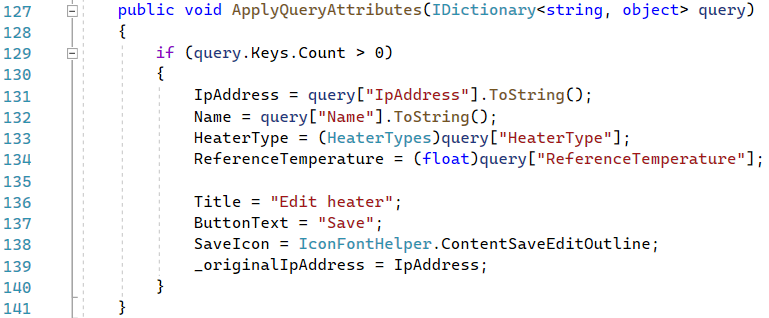
\includegraphics[width=0.72\textwidth]{obrazky-figures/code-applyqueryattributes.png}
\caption{Viewmodel pro použití URI navigace implementuje rozhraní {\it IQueryAttributable} a jeho metodu {\it ApplyQueryAttributes} z jejíhož slovníkového parametru lze získat například informace o editovaném topení. Na stránku je možné se navigovat i bez parametrů, v tomto případě se pak jedná o přidání.}
\end{figure}

\begin{figure}[hbt]
\centering
\frame{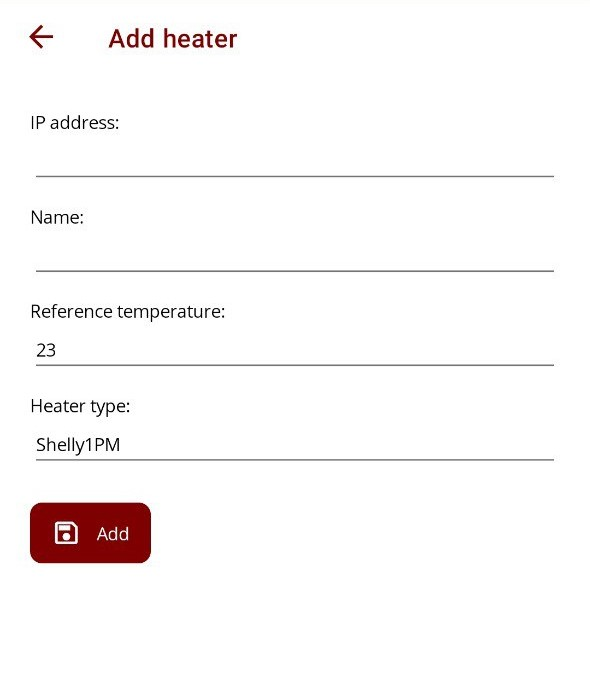
\includegraphics[width=0.32\textwidth]{obrazky-figures/screenshots/2-add.jpg}}
\frame{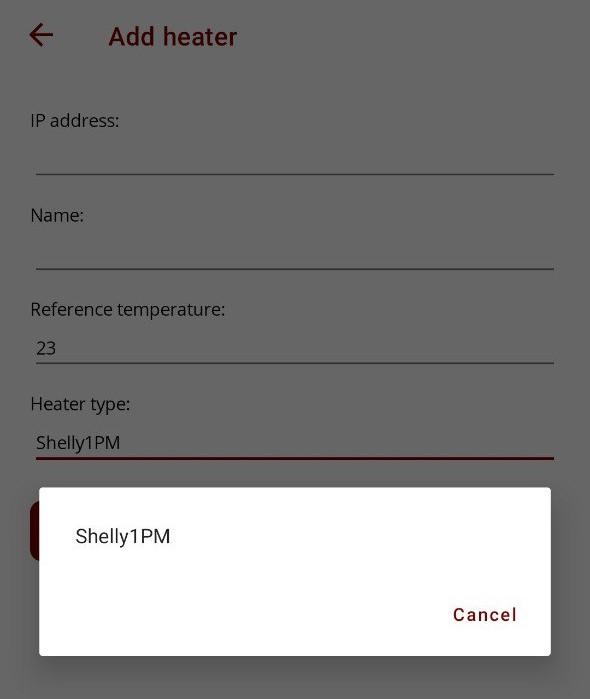
\includegraphics[width=0.32\textwidth]{obrazky-figures/screenshots/2-add-type.jpg}}
\frame{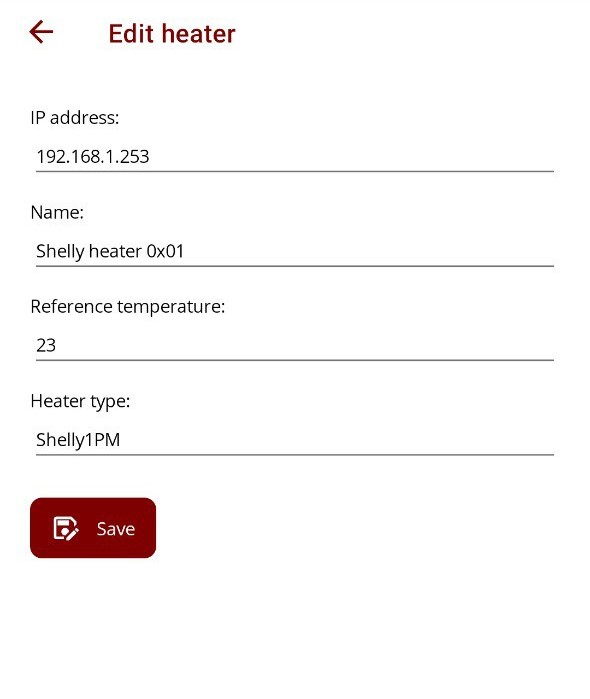
\includegraphics[width=0.32\textwidth]{obrazky-figures/screenshots/2-edit.jpg}}
\caption{Uživatelské rozhraní {\it AddHeaterPage} má v případě přidávání textová pole prázdná a v případě editace vyplněná dle vybraného topení. Výběr typu topení je zde pro případnou budoucí podporu více typů předpřipraven ve značce {\it Picker}.}
\end{figure}

Další částí pro samotné monitorování stavu topení je stránka detailu, která se zobrazí po kliknutí na položku v seznamu registrovaných topení na úvodní stránce {\it HeatersPage}. K této stránce patří viewmodel {\it HeaterDetailViewModel}, který implementuje podporu URI navigace s parametrem IP adresy topení. Ta je použita jako parametr metody {\it GetHeaterDataAsync}, která pomocí HTTP metody {\it GET} stáhne data o daném topení a deserializuje je do objektu typu {\it HeaterDetailModel}.

Nahoře na stránce se nachází tlačítka s akcemi nad topením pro znovunačtení aktuálních informací o topení, navigaci na editační stránku topení a jeho smazání. Znovunačtení je provedeno voláním metody {\it ReLoad}, která opět volá {\it GetHeaterDataAsync} s parametrem IP adresy aktuálně zobrazeného topení. Editační tlačítko naviguje pomocí {\it Shell} na stránku {\it AddHeaterPage}, které předá parametry k editaci. Tlačítko smazání zobrazí dialog o potvzení smazání, a pokud je zvolena možnost {\it ''Ano''} posílá HTTP požadavek metodou {\it DELETE}. Zvolením {\it ''Ne''} je dialog uzavřen a požadavek na smazání serveru není odeslán.

\begin{figure}[hbt]
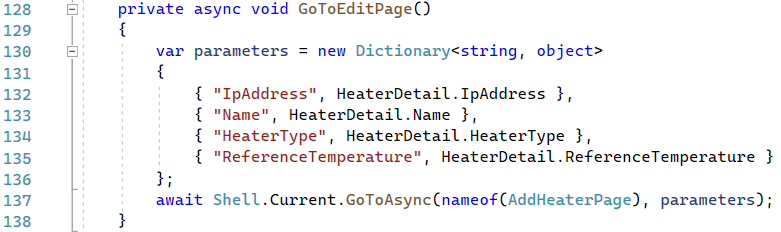
\includegraphics[width=0.72\textwidth]{obrazky-figures/code-gotoedit.png}
\caption{Metoda {\it HeaterDetailViewModel} pro URI navigaci na editační stránku topení.}
\end{figure}

Tato stránka má dvě varianty na základě platformy (mobilní pro Android a iOS, a desktopovou pro ostatní), jak již bylo zmíněno u obrázku \ref{appshellprovider}. Kvůli tomuto rozdělení je kód pro zobrazení informací o topení extrahován do pohledu {\it HeaterDetailView} a {\it HeaterChartsView}. Tímto se stávají znovupoužitelnými a zamezuje se kopírování kódu.

{\it HeaterDetailView} zobrazuje informace z objektu typu {\it HeaterDetailModel}, který mu je předán jako {\it BindingContext}.

\pagebreak

{\it HeaterChartsView} obsahuje grafy, které umožní uživateli zobrazit si a mít přehled o historii teploty v místnosti, kde je topení umístěno, a spotřebě elektrické energie. V aplikaci jsou pro tento účel využity grafy z knihovny {\it Syncfusion.Maui.Charts} dle \cite{maui-charts}. Tento pohled obsahuje viewmodel typu {\it HeaterChartsViewModel}, ve kterém jsou uloženy kolekce s daty pro zobrazení v grafech.

Pro výběr časového období a následného stažení dat byl navíc přidán pohled {\it PeriodSelectorView}. Ten pracuje s vlastním viewmodelem typu {\it PeriodSelectorViewModel}, který v parametru konstruktoru přijímá delegát akce. Tlačítko pro načtení dat historie volá tento delegát po svém stisknutí. Předaná metoda v případě {\it HeaterChartsViewModel} použije HTTP metodu {\it GET} pro stažení dat ze zvoleného časového období o položkách databáze teploty a spotřeby. Získaná data jsou následně uložena do kolekcí, které mají datové vazby na grafy z knihovny {\it Syncfusion.Maui.Charts}.

\begin{figure}[hbt]
\centering
\frame{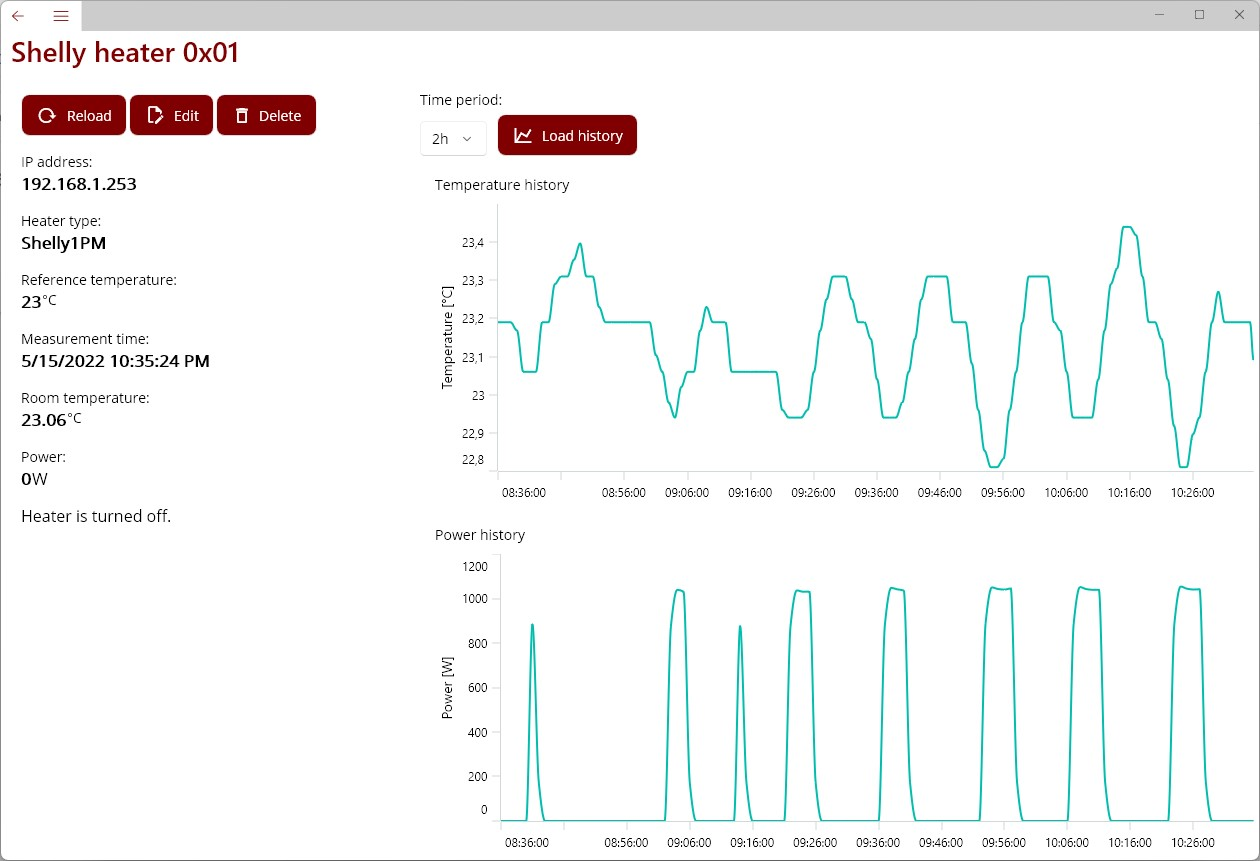
\includegraphics[width=0.9\textwidth]{obrazky-figures/screenshots/3-heaterdetail.png}}
\caption{Desktopové uživatelské rozhraní detailu topení zobrazuje grafy v {\it HeaterChartsView} na pravé straně od informací o topení v {\it HeaterDetailView} a tlačítky s dostupnými akcemi. Pro mobilní zařízení jsou z důvodu úzké obrazovky tyto pohledy umístěny pod sebou.}
\end{figure}

\subsection{Zobrazení dat o počasí}
O zobrazení dat o venkovním počasí se stará stránka {\it WeatherPage}. K této stránce patří viewmodel typu {\it WeatherViewModel}, který se po své inicializaci pomocí HTTP metody {\it GET} pokusí získat informace o aktuální venkovní teplotě. Tato stránka také pro zobrazení historie počasí obsahuje grafy z knihovny {\it Syncfusion.Maui.Charts} dle \cite{maui-charts} a volbu časového období pomocí {\it PeriodSelectorView}.

\begin{figure}[hbt]
\centering
\frame{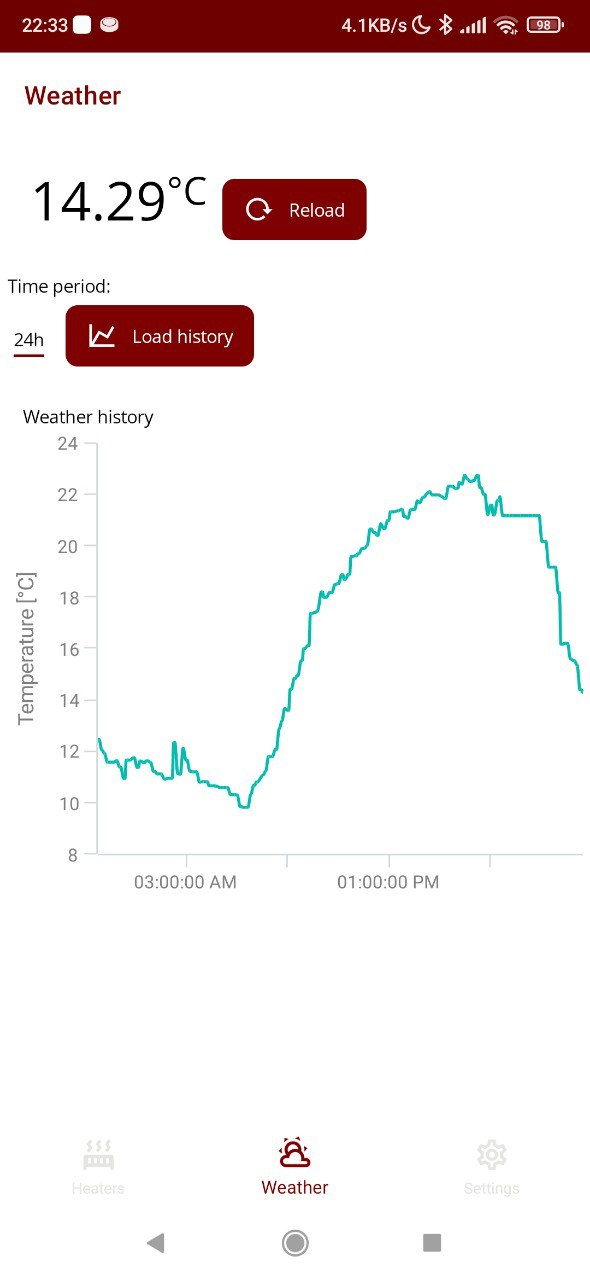
\includegraphics[height=8.6cm]{obrazky-figures/screenshots/4-weather.png}}
\frame{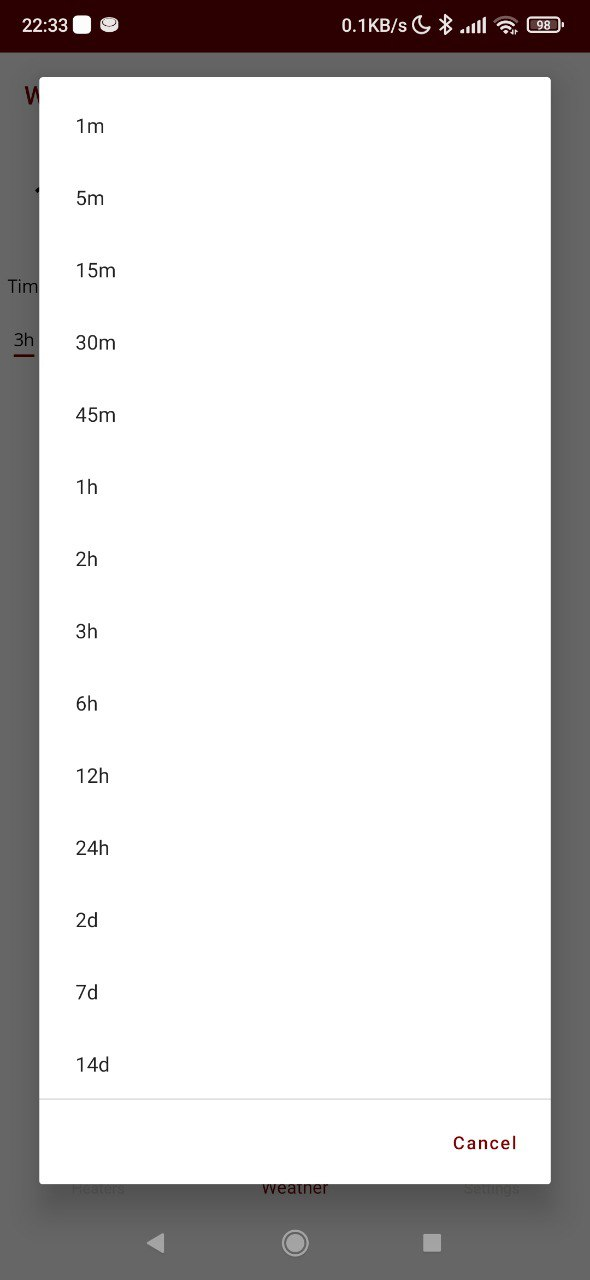
\includegraphics[height=8.6cm]{obrazky-figures/screenshots/4-periods-select.png}}
\caption{Stránka zobrazení dat o počasí a výběr časového období.}
\end{figure}


\subsection{Stránka nastavení}


\subsection{Pomocné třídy}
Converters, Helpers

\begin{figure}[hbt]
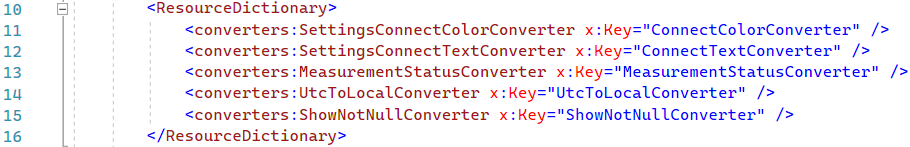
\includegraphics[width=0.85\textwidth]{obrazky-figures/code-maui-converters0.png}
\caption{}
\end{figure}

\begin{figure}[hbt]
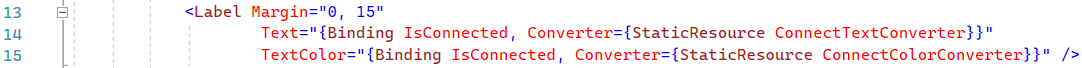
\includegraphics[width=\textwidth]{obrazky-figures/code-maui-converters1.png}
\caption{}
\end{figure}

\begin{figure}[hbt]
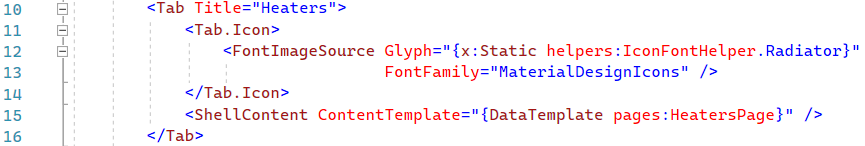
\includegraphics[width=0.81\textwidth]{obrazky-figures/code-maui-icons.png}
\caption{}
\end{figure}

\section{Předpověď strojovým učením}
Úvod k {\it SmartHeaterModel}

\subsection{Trénovací data}
Generování

Data

\subsection{Model strojového učení}


\subsection{Algoritmus rozhodování o ovládání topení}


\section{Sledování chování systému}
Jak to sleduju v StatsCollectorInvocable atd...


\subsection{Původní termostat}



\subsection{Ovládání strojovým učením}


\chapter{Závěr}
\label{zaver}

Integrace do populární platformy typu Home Assistant, Telegram Bot, přidat krom vytápění i chlazení. Možné rozšíření podpory dalších zařízení krom Shelly 1PM, například dříve zmíněnými chytrými přímotopy.

%===============================================================================
